\documentclass[a4paper, openany]{memoir}

\usepackage[utf8]{inputenc}
\usepackage[T1]{fontenc} 
\usepackage[english]{babel}
\usepackage{fancyhdr}
\usepackage{float}
\usepackage{amsmath}
\usepackage{amsthm}
\usepackage{amssymb}
\usepackage[bookmarksopen=true,bookmarksopenlevel=2]{hyperref}
\usepackage{tikz}
\usepackage{indentfirst}

\usepackage{listings}
\usepackage{xcolor}

\pagestyle{fancy}
\fancyhf{}
\fancyhead[LE]{\leftmark}
\fancyhead[RO]{\rightmark}
\fancyhead[RE, LO]{Programming Languages}
\fancyfoot[LE, RO]{\thepage}
\fancyfoot[RE, LO]{Pete Gautam}

\renewcommand{\headrulewidth}{1.5pt}

\usetikzlibrary{shapes}

\definecolor{codegreen}{rgb}{0,0.6,0}
\definecolor{codegray}{rgb}{0.5,0.5,0.5}
\definecolor{codepurple}{rgb}{0.58,0,0.82}
\definecolor{backcolour}{rgb}{0.95,0.95,0.92}

\lstdefinestyle{thestyle}{
    backgroundcolor=\color{backcolour},
    basicstyle=\ttfamily\footnotesize,
    keywordstyle=\color{red!80}\bfseries,
    ndkeywordstyle=\color{blue!80}\bfseries,
    identifierstyle=\color{black},
    commentstyle=\color{codegreen},
    stringstyle=\color{codepurple},
    breakatwhitespace=false,
    breaklines=true,
    captionpos=b,
    keepspaces=true,
    numberstyle=\tiny\color{codegray},
    numbers=left,
    numbersep=2pt,
    showspaces=false,
    showstringspaces=false,
    showtabs=false,          
    tabsize=2
}

\lstdefinelanguage{SVM}{ 
    keywords={LOADC, STOREG, LOADG, JUMPF, JUMP, HALT, CALL, RETURN},
    ndkeywords={COMPLT, COMPGT, ADD, SUB, MUL, DIV},
    sensitive=true,
    comment=[l]{//},
    morecomment=[s]{/*}{*/},
    morestring=[b]',
    morestring=[b]"
}

\lstdefinelanguage{fun}{ 
    keywords={func, while, if, proc, return, read, write},
    ndkeywords={int, char, bool, List, String, Node, Queue, Set, Trie, void, true, false},
    sensitive=true,
    comment=[l]{\#},
    % morecomment=[s]{##}{##},
    morestring=[b]',
    morestring=[b]"
}

\lstdefinelanguage{calc}{ 
    keywords={set, put},
    ndkeywords={},
    sensitive=true,
    comment=[l]{//},
    morecomment=[s]{/*}{*/},
    morestring=[b]',
    morestring=[b]"
}

\lstset{style=thestyle}

\chapterstyle{thatcher}
\setcounter{chapter}{1}

\begin{document}
\chapter{Implementation}
\section{Compilers and Interpreters}
An $S \to T$ translator accepts code expressed in one language $S$ (the source language), and translates it to equivalent code expressed in another language $T$ (the target language). Examples of translators include:
\begin{itemize}
    \item compilers, which translate high-level PL code to low level code, e.g. Java $\to$ JVM, C $\to$ x86as (x86 assembly code) and C $\to$ x86 (machine code).
    \item assemblers, which translate assembly language to the corresponding machine code, e.g. x86as $\to$ x86.
    \item high-level translators, or transpilers, which translate code in one high-level PL to code in another high level PL, e.g. Java $\to$ C.
    \item decompilers, or disassemblers, which translate low-level code to high(er)-level PL code, e.g. JVM $\to$ Java and x86 $\to$ x86as.
\end{itemize}

An $S$ interpreter accepts code expressed in language $S$, and immediately executes that code. That is, there is no intermediate object code generated. It works by fetching, analysing and executing one instruction at a time. If an instruction is fetched repeatedly, it will be analysed repeatedly. This is time consuming unless instructions have very simple formats.

Interpreting a program is slower than executing native machine code. Moreover, interpreting a high-level language is much slower than interpreting an intermediate-level language, such as JVM code. On the other hand, interpreting a program cuts out compile-time.

Interpretation is sensible when:
\begin{itemize}
    \item a user is entering instructions interactively and wishes to see the results of each instruction before entering the next one;
    \item the program is to be used once and then discarded (meaning that the execution speed doesn't matter);
    \item each instruction will be executed only once or a few times;
    \item the instructions have very simple formats;
    \item the program code is required to be highly portable.
\end{itemize}

Some interpreters are:
\begin{itemize}
    \item Unix command language interpreter (shell). Here, the user enters one command at a time. The shell reads the command, parses it to determine the command name and arguments, and executes it.
    \item JVM (Java virtual machine) interpreter. A JVM program consists of bytecodes. The interpreter fetches, decodes and executes one bytecode at a time.
\end{itemize}

There is a big difference between compilers and interpreters. A compiler translates source code to object code. It does not execute the source or object code. On the other hand, an interpreter executes source code one instruction at a time. It does not translate the source code.

\subsection{Tombstone diagrams}
We can use tombstone diagrams to represent programs, interpreters, compilers and hardware. We have the following symbols available:
\begin{itemize}
    \item The following figure is used to denote a program.
    \begin{figure}[H]
        \centering
        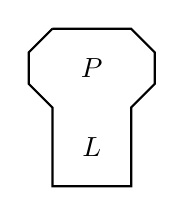
\begin{tikzpicture}
        \draw[thick] (0, 0) -- (1, 0) 
            -- (1.3, -0.3)
            -- (1.3, -0.7)
            -- (1, -1)
            -- (1, -2)
            -- (0, -2)
            -- (0, -1)
            -- (-0.3, -0.7)
            -- (-0.3, -0.3)
            -- (0, 0);
            \node at (0.5, -0.5) {$P$};
            \node at (0.5, -1.5) {$L$};
        \end{tikzpicture}
        \caption{A tombstone diagram for a program $P$ in language $L$.}
    \end{figure}
    
    \item The following figure is used to denote a translator.
    \begin{figure}[H]
        \centering
        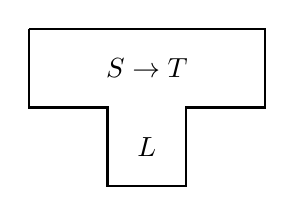
\begin{tikzpicture}
        \draw[thick] (0, 0) -- (3, 0)
            -- (3, -1)
            -- (2, -1)
            -- (2, -2)
            -- (1, -2)
            -- (1, -1)
            -- (0, -1)
            -- (0, 0);
        \node at (1.5, -0.5) {$S \to T$};
        \node at (1.5, -1.5) {$L$};
        \end{tikzpicture}
        \caption{An $S \to T$ translator expressed in the language $L$.}
    \end{figure}
    
    \item The following figure is used to denote an interpreter
    \begin{figure}[H]
        \centering
        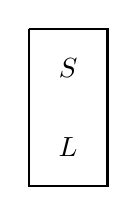
\begin{tikzpicture}
        \draw[thick] (0, 0) -- (1, 0)
            -- (1, -2)
            -- (0, -2)
            -- (0, 0);
        \node at (0.5, -0.5) {$S$};
        \node at (0.5, -1.5) {$L$};
        \end{tikzpicture}
        \caption{An $S$ interpreter in the language $L$.}
    \end{figure}
    
    \item The following figure is used to denote a hardware.
    \begin{figure}[H]
        \centering
        
\begin{tikzpicture}
        \draw[thick] (0, 0) -- (1, 0)
            -- (1, -0.3)
            -- (0.5, -1)
            -- (0, -0.3)
            -- (0, 0);
        \node at (0.5, -0.3) {$M$};
        \end{tikzpicture}
        \caption{A machine $M$ which can only execute $M$'s machine code.}
    \end{figure}
\end{itemize}

We will now look at some concrete examples of tombstone diagrams. 
\begin{itemize}
    \item We can denote the the program \texttt{sort} written in 3 different languages- Java, JVM and x86.
    \begin{figure}[H]
        \centering
        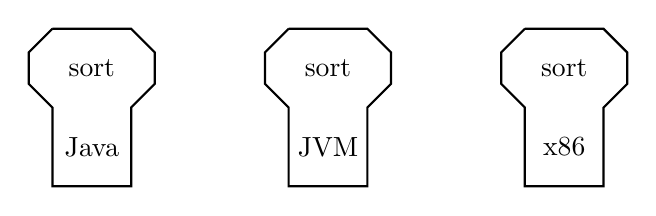
\begin{tikzpicture}
            \draw[thick] (0, 0) -- (1, 0) 
            -- (1.3, -0.3)
            -- (1.3, -0.7)
            -- (1, -1)
            -- (1, -2)
            -- (0, -2)
            -- (0, -1)
            -- (-0.3, -0.7)
            -- (-0.3, -0.3)
            -- (0, 0);
            \node at (0.5, -0.5) {sort};
            \node at (0.5, -1.5) {Java};
            
            \draw[thick] (0+3, 0) -- (1+3, 0) 
            -- (1.3+3, -0.3)
            -- (1.3+3, -0.7)
            -- (1+3, -1)
            -- (1+3, -2)
            -- (0+3, -2)
            -- (0+3, -1)
            -- (-0.3+3, -0.7)
            -- (-0.3+3, -0.3)
            -- (0+3, 0);
            \node at (0.5+3, -0.5) {sort};
            \node at (0.5+3, -1.5) {JVM};
            
            \draw[thick] (0+6, 0) -- (1+6, 0) 
            -- (1.3+6, -0.3)
            -- (1.3+6, -0.7)
            -- (1+6, -1)
            -- (1+6, -2)
            -- (0+6, -2)
            -- (0+6, -1)
            -- (-0.3+6, -0.7)
            -- (-0.3+6, -0.3)
            -- (0+6, 0);
            \node at (0.5+6, -0.5) {sort};
            \node at (0.5+6, -1.5) {x86};
        \end{tikzpicture}
    \end{figure}
    
    \item We can denote the interpreters: a JVM interpreter in C, a JVM interpreter in x86 and a Ruby interpreter in x86.
    \begin{figure}[H]
        \centering
        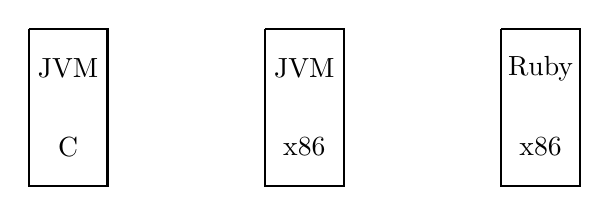
\begin{tikzpicture}
        \draw[thick] (0, 0) -- (1, 0)
            -- (1, -2)
            -- (0, -2)
            -- (0, 0);
        \node at (0.5, -0.5) {JVM};
        \node at (0.5, -1.5) {C};
    
    
        \draw[thick] (0+3, 0) -- (1+3, 0)
            -- (1+3, -2)
            -- (0+3, -2)
            -- (0+3, 0);
        \node at (0.5+3, -0.5) {JVM};
        \node at (0.5+3, -1.5) {x86};
    
    
        \draw[thick] (0+6, 0) -- (1+6, 0)
            -- (1+6, -2)
            -- (0+6, -2)
            -- (0+6, 0);
        \node at (0.5+6, -0.5) {Ruby};
        \node at (0.5+6, -1.5) {x86};
        \end{tikzpicture}
    \end{figure}
    
    \item We can denote the translators: a Java $\to$ JVM compiler in Java, a Java $\to$ C transpiler, an x86as $\to$ x86 assembler in x86, and a JVM $\to$ Java decompiler in C.
    \begin{figure}[H]
        \centering
        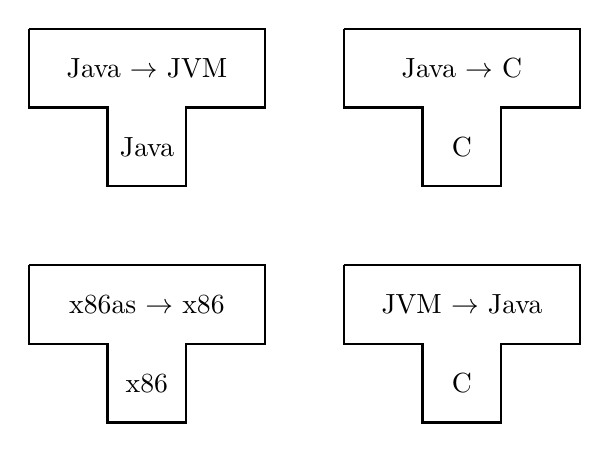
\begin{tikzpicture}
        \draw[thick] (0, 0) -- (3, 0)
            -- (3, -1)
            -- (2, -1)
            -- (2, -2)
            -- (1, -2)
            -- (1, -1)
            -- (0, -1)
            -- (0, 0);
        \node at (1.5, -0.5) {Java $\to$ JVM};
        \node at (1.5, -1.5) {Java};
        
        \draw[thick] (0+4, 0) -- (3+4, 0)
            -- (3+4, -1)
            -- (2+4, -1)
            -- (2+4, -2)
            -- (1+4, -2)
            -- (1+4, -1)
            -- (0+4, -1)
            -- (0+4, 0);
        \node at (1.5+4, -0.5) {Java $\to$ C};
        \node at (1.5+4, -1.5) {C};
        
        \draw[thick] (0, 0-3) -- (3, 0-3)
            -- (3, -1-3)
            -- (2, -1-3)
            -- (2, -2-3)
            -- (1, -2-3)
            -- (1, -1-3)
            -- (0, -1-3)
            -- (0, 0-3);
        \node at (1.5, -0.5-3) {x86as $\to$ x86};
        \node at (1.5, -1.5-3) {x86};
        
        \draw[thick] (0+4, 0-3) -- (3+4, 0-3)
            -- (3+4, -1-3)
            -- (2+4, -1-3)
            -- (2+4, -2-3)
            -- (1+4, -2-3)
            -- (1+4, -1-3)
            -- (0+4, -1-3)
            -- (0+4, 0-3);
        \node at (1.5+4, -0.5-3) {JVM $\to$ Java};
        \node at (1.5+4, -1.5-3) {C};
        \end{tikzpicture}
    \end{figure}
\end{itemize}

We can use tombstone diagrams to run programs. Given a program $P$ expressed in $M$ machine code, we can run $P$ on machine $M$.
\begin{figure}[H]
    \centering
    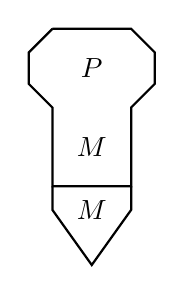
\begin{tikzpicture}
    \draw[thick] (0, 0) -- (1, 0) 
        -- (1.3, -0.3)
        -- (1.3, -0.7)
        -- (1, -1)
        -- (1, -2)
        -- (0, -2)
        -- (0, -1)
        -- (-0.3, -0.7)
        -- (-0.3, -0.3)
        -- (0, 0);
    \node at (0.5, -0.5) {$P$};
    \node at (0.5, -1.5) {$M$};

    \draw[thick] (1, 0-2) -- (1, -0.3-2)
        -- (0.5, -1-2)
        -- (0, -0.3-2)
        -- (0, 0-2);
    \node at (0.5, -0.3-2) {$M$};
    \end{tikzpicture}
    \caption{Running a program $P$ written in $M$.}
\end{figure}
\noindent Note that the two $M$'s must match for the program to run. So, we can run the sort program in x86 and ARM given the right hardware.
\begin{figure}[H]
    \centering
    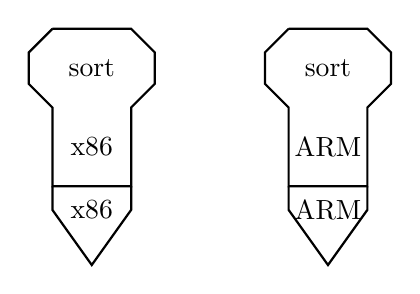
\begin{tikzpicture}
    \draw[thick] (0, 0) -- (1, 0) 
        -- (1.3, -0.3)
        -- (1.3, -0.7)
        -- (1, -1)
        -- (1, -2)
        -- (0, -2)
        -- (0, -1)
        -- (-0.3, -0.7)
        -- (-0.3, -0.3)
        -- (0, 0);
    \node at (0.5, -0.5) {sort};
    \node at (0.5, -1.5) {x86};

    \draw[thick] (1, 0-2) -- (1, -0.3-2)
        -- (0.5, -1-2)
        -- (0, -0.3-2)
        -- (0, 0-2);
    \node at (0.5, -0.3-2) {x86};
    
    \draw[thick] (0+3, 0) -- (1+3, 0) 
        -- (1.3+3, -0.3)
        -- (1.3+3, -0.7)
        -- (1+3, -1)
        -- (1+3, -2)
        -- (0+3, -2)
        -- (0+3, -1)
        -- (-0.3+3, -0.7)
        -- (-0.3+3, -0.3)
        -- (0+3, 0);
    \node at (0.5+3, -0.5) {sort};
    \node at (0.5+3, -1.5) {ARM};

    \draw[thick] (1+3, 0-2) -- (1+3, -0.3-2)
        -- (0.5+3, -1-2)
        -- (0+3, -0.3-2)
        -- (0+3, 0-2);
    \node at (0.5+3, -0.3-2) {ARM};
    \end{tikzpicture}
\end{figure}
\noindent However, the following are not possible since the language of the program doesn't match the hardware.
\begin{figure}[H]
    \centering
    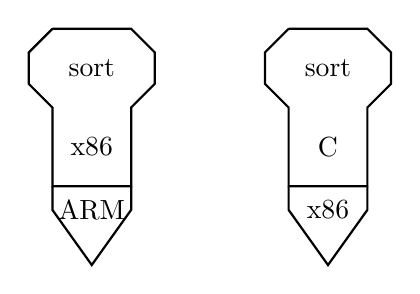
\begin{tikzpicture}
    \draw[thick] (0, 0-4) -- (1, 0-4) 
        -- (1.3, -0.3-4)
        -- (1.3, -0.7-4)
        -- (1, -1-4)
        -- (1, -2-4)
        -- (0, -2-4)
        -- (0, -1-4)
        -- (-0.3, -0.7-4)
        -- (-0.3, -0.3-4)
        -- (0, 0-4);
    \node at (0.5, -0.5-4) {sort};
    \node at (0.5, -1.5-4) {x86};

    \draw[thick] (1, 0-2-4) -- (1, -0.3-2-4)
        -- (0.5, -1-2-4)
        -- (0, -0.3-2-4)
        -- (0, 0-2-4);
    \node at (0.5, -0.3-2-4) {ARM};
    
    \draw[thick] (0+3, 0-4) -- (1+3, 0-4) 
        -- (1.3+3, -0.3-4)
        -- (1.3+3, -0.7-4)
        -- (1+3, -1-4)
        -- (1+3, -2-4)
        -- (0+3, -2-4)
        -- (0+3, -1-4)
        -- (-0.3+3, -0.7-4)
        -- (-0.3+3, -0.3-4)
        -- (0+3, 0-4);
    \node at (0.5+3, -0.5-4) {sort};
    \node at (0.5+3, -1.5-4) {C};

    \draw[thick] (1+3, 0-2-4) -- (1+3, -0.3-2-4)
        -- (0.5+3, -1-2-4)
        -- (0+3, -0.3-2-4)
        -- (0+3, 0-2-4);
    \node at (0.5+3, -0.3-2-4) {x86};
    \end{tikzpicture}
\end{figure}

We can also show the translation of a program via tombstone diagrams. Given an $S \to T$ translator, expressed in $M$ machine code, and a program $P$ expressed in language $S$, we can translate $P$ to language $T$.
\begin{figure}[H]
    \centering
    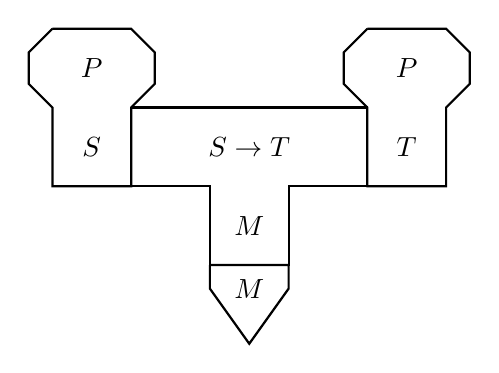
\begin{tikzpicture}
    \draw[thick] (0, 0) -- (1, 0) 
        -- (1.3, -0.3)
        -- (1.3, -0.7)
        -- (1, -1)
        -- (1, -2)
        -- (0, -2)
        -- (0, -1)
        -- (-0.3, -0.7)
        -- (-0.3, -0.3)
        -- (0, 0);
        \node at (0.5, -0.5) {$P$};
        \node at (0.5, -1.5) {$S$};
        
      \draw[thick] (0+1, 0-1) -- (3+1, 0-1)
        -- (3+1, -1-1)
        -- (2+1, -1-1)
        -- (2+1, -2-1)
        -- (1+1, -2-1)
        -- (1+1, -1-1)
        -- (0+1, -1-1)
        -- (0+1, 0-1);
    \node at (1.5+1, -0.5-1) {$S \to T$};
    \node at (1.5+1, -1.5-1) {$M$};

    \draw[thick] (0+4, 0) -- (1+4, 0) 
        -- (1.3+4, -0.3)
        -- (1.3+4, -0.7)
        -- (1+4, -1)
        -- (1+4, -2)
        -- (0+4, -2)
        -- (0+4, -1)
        -- (-0.3+4, -0.7)
        -- (-0.3+4, -0.3)
        -- (0+4, 0);
        \node at (0.5+4, -0.5) {$P$};
        \node at (0.5+4, -1.5) {$T$};

    \draw[thick] (0+2, 0-3) -- (1+2, 0-3)
        -- (1+2, -0.3-3)
        -- (0.5+2, -1-3)
        -- (0+2, -0.3-3)
        -- (0+2, 0-3);
    \node at (0.5+2, -0.3-3) {$M$};
    \end{tikzpicture}
\end{figure}
\noindent Note that the PLs must match the source and the target languages of the translator. Also, the language of the translator must match the language of the hardware. An example of this is given below- compiling the sort program from C to x86.
\begin{figure}[H]
    \centering
    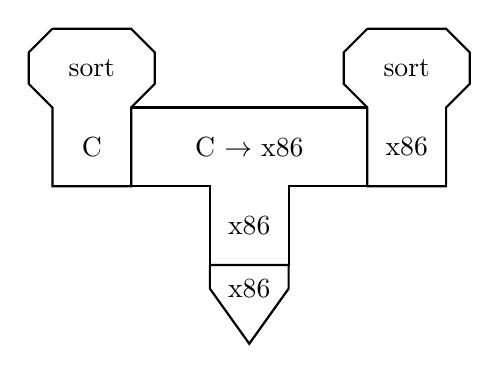
\begin{tikzpicture}
    \draw[thick] (0, 0) -- (1, 0) 
        -- (1.3, -0.3)
        -- (1.3, -0.7)
        -- (1, -1)
        -- (1, -2)
        -- (0, -2)
        -- (0, -1)
        -- (-0.3, -0.7)
        -- (-0.3, -0.3)
        -- (0, 0);
        \node at (0.5, -0.5) {sort};
        \node at (0.5, -1.5) {C};
        
      \draw[thick] (0+1, 0-1) -- (3+1, 0-1)
        -- (3+1, -1-1)
        -- (2+1, -1-1)
        -- (2+1, -2-1)
        -- (1+1, -2-1)
        -- (1+1, -1-1)
        -- (0+1, -1-1)
        -- (0+1, 0-1);
    \node at (1.5+1, -0.5-1) {C $\to$ x86};
    \node at (1.5+1, -1.5-1) {x86};

    \draw[thick] (0+4, 0) -- (1+4, 0) 
        -- (1.3+4, -0.3)
        -- (1.3+4, -0.7)
        -- (1+4, -1)
        -- (1+4, -2)
        -- (0+4, -2)
        -- (0+4, -1)
        -- (-0.3+4, -0.7)
        -- (-0.3+4, -0.3)
        -- (0+4, 0);
        \node at (0.5+4, -0.5) {sort};
        \node at (0.5+4, -1.5) {x86};

    \draw[thick] (0+2, 0-3) -- (1+2, 0-3)
        -- (1+2, -0.3-3)
        -- (0.5+2, -1-3)
        -- (0+2, -0.3-3)
        -- (0+2, 0-3);
    \node at (0.5+2, -0.3-3) {x86};
    \end{tikzpicture}
\end{figure}
\noindent This represents the compilation of the program. We can later run the object program on an x86, which is depicted by the tombstone diagram below.
\begin{figure}[H]
    \centering
    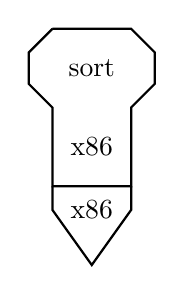
\begin{tikzpicture}
    \draw[thick] (0+3, 0-4) -- (1+3, 0-4) 
        -- (1.3+3, -0.3-4)
        -- (1.3+3, -0.7-4)
        -- (1+3, -1-4)
        -- (1+3, -2-4)
        -- (0+3, -2-4)
        -- (0+3, -1-4)
        -- (-0.3+3, -0.7-4)
        -- (-0.3+3, -0.3-4)
        -- (0+3, 0-4);
    \node at (0.5+3, -0.5-4) {sort};
    \node at (0.5+3, -1.5-4) {x86};

    \draw[thick] (1+3, 0-2-4) -- (1+3, -0.3-2-4)
        -- (0.5+3, -1-2-4)
        -- (0+3, -0.3-2-4)
        -- (0+3, 0-2-4);
    \node at (0.5+3, -0.3-2-4) {x86};
    \end{tikzpicture}
\end{figure}
\noindent This represents the runtime of the program.

We could break the compilation into 2 steps. For example, we can have a C $\to$ x86as compiler, and an x86 assembler. Then, we can use them to compile a program in C into x86 machine code, in 2 stages.
\begin{figure}[H]
    \centering
    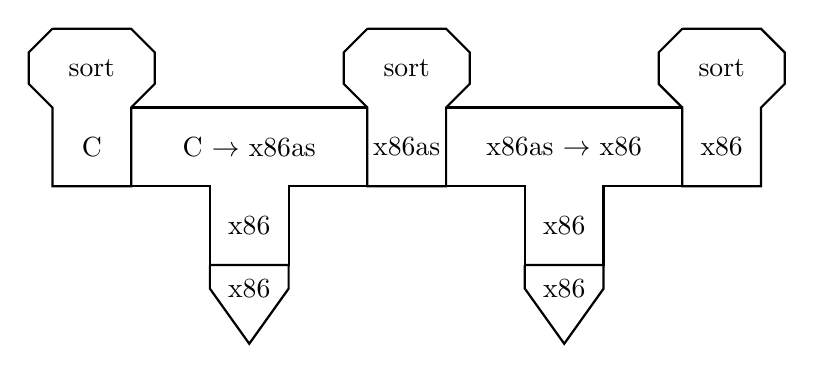
\begin{tikzpicture}
    \draw[thick] (0, 0) -- (1, 0) 
        -- (1.3, -0.3)
        -- (1.3, -0.7)
        -- (1, -1)
        -- (1, -2)
        -- (0, -2)
        -- (0, -1)
        -- (-0.3, -0.7)
        -- (-0.3, -0.3)
        -- (0, 0);
        \node at (0.5, -0.5) {sort};
        \node at (0.5, -1.5) {C};
        
      \draw[thick] (0+1, 0-1) -- (3+1, 0-1)
        -- (3+1, -1-1)
        -- (2+1, -1-1)
        -- (2+1, -2-1)
        -- (1+1, -2-1)
        -- (1+1, -1-1)
        -- (0+1, -1-1)
        -- (0+1, 0-1);
    \node at (1.5+1, -0.5-1) {C $\to$ x86as};
    \node at (1.5+1, -1.5-1) {x86};

    \draw[thick] (0+4, 0) -- (1+4, 0) 
        -- (1.3+4, -0.3)
        -- (1.3+4, -0.7)
        -- (1+4, -1)
        -- (1+4, -2)
        -- (0+4, -2)
        -- (0+4, -1)
        -- (-0.3+4, -0.7)
        -- (-0.3+4, -0.3)
        -- (0+4, 0);
        \node at (0.5+4, -0.5) {sort};
        \node at (0.5+4, -1.5) {x86as};

    \draw[thick] (0+2, 0-3) -- (1+2, 0-3)
        -- (1+2, -0.3-3)
        -- (0.5+2, -1-3)
        -- (0+2, -0.3-3)
        -- (0+2, 0-3);
    \node at (0.5+2, -0.3-3) {x86};
        
     \draw[thick] (0+5, 0-1) -- (3+5, 0-1)
        -- (3+5, -1-1)
        -- (2+5, -1-1)
        -- (2+5, -2-1)
        -- (1+5, -2-1)
        -- (1+5, -1-1)
        -- (0+5, -1-1)
        -- (0+5, 0-1);
    \node at (1.5+5, -0.5-1) {x86as $\to$ x86};
    \node at (1.5+5, -1.5-1) {x86};

    \draw[thick] (0+8, 0) -- (1+8, 0) 
        -- (1.3+8, -0.3)
        -- (1.3+8, -0.7)
        -- (1+8, -1)
        -- (1+8, -2)
        -- (0+8, -2)
        -- (0+8, -1)
        -- (-0.3+8, -0.7)
        -- (-0.3+8, -0.3)
        -- (0+8, 0);
        \node at (0.5+8, -0.5) {sort};
        \node at (0.5+8, -1.5) {x86};

    \draw[thick] (0+6, 0-3) -- (1+6, 0-3)
        -- (1+6, -0.3-3)
        -- (0.5+6, -1-3)
        -- (0+6, -0.3-3)
        -- (0+6, 0-3);
    \node at (0.5+6, -0.3-3) {x86};
    \end{tikzpicture}
\end{figure}

We can compile a compiler. Given a C $\to$ x86 compiler, we can use it to compile any C program into x86 machine code. In particular, we can compile a compiler expressed in C, e.g. compiling a Java $\to$ JVM compiler written in C to a Java $\to$ JVM compiler in x86.
\begin{figure}[H]
    \centering
    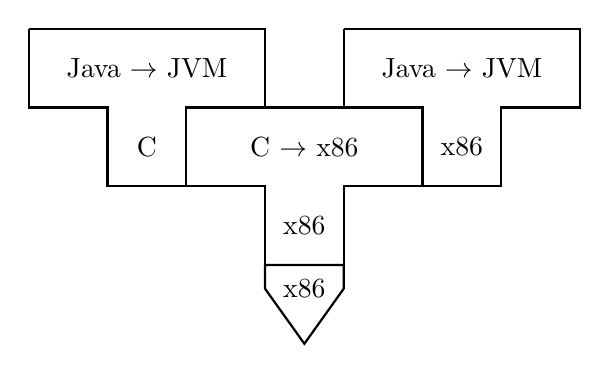
\begin{tikzpicture}
    \draw[thick] (0-1, 0) -- (3-1, 0)
        -- (3-1, -1)
        -- (2-1, -1)
        -- (2-1, -2)
        -- (1-1, -2)
        -- (1-1, -1)
        -- (0-1, -1)
        -- (0-1, 0);
    \node at (1.5-1, -0.5) {Java $\to$ JVM};
    \node at (1.5-1, -1.5) {C};
        
      \draw[thick] (0+1, 0-1) -- (3+1, 0-1)
        -- (3+1, -1-1)
        -- (2+1, -1-1)
        -- (2+1, -2-1)
        -- (1+1, -2-1)
        -- (1+1, -1-1)
        -- (0+1, -1-1)
        -- (0+1, 0-1);
    \node at (1.5+1, -0.5-1) {C $\to$ x86};
    \node at (1.5+1, -1.5-1) {x86};

    \draw[thick] (0+3, 0) -- (3+3, 0)
        -- (3+3, -1)
        -- (2+3, -1)
        -- (2+3, -2)
        -- (1+3, -2)
        -- (1+3, -1)
        -- (0+3, -1)
        -- (0+3, 0);
    \node at (1.5+3, -0.5) {Java $\to$ JVM};
    \node at (1.5+3, -1.5) {x86};

    \draw[thick] (0+2, 0-3) -- (1+2, 0-3)
        -- (1+2, -0.3-3)
        -- (0.5+2, -1-3)
        -- (0+2, -0.3-3)
        -- (0+2, 0-3);
    \node at (0.5+2, -0.3-3) {x86};
    \end{tikzpicture}
\end{figure}
\noindent For this to be possible, we require the relevant languages to match. So, the following is possible.
\begin{figure}[H]
    \centering
    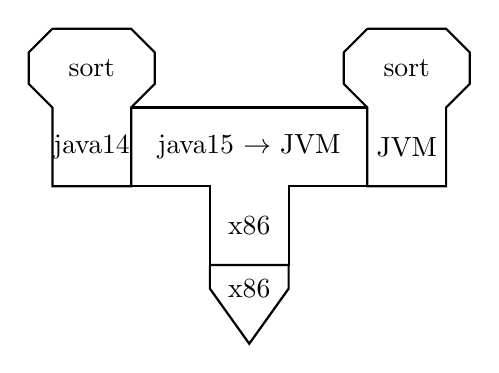
\begin{tikzpicture}
    \draw[thick] (0, 0) -- (1, 0) 
        -- (1.3, -0.3)
        -- (1.3, -0.7)
        -- (1, -1)
        -- (1, -2)
        -- (0, -2)
        -- (0, -1)
        -- (-0.3, -0.7)
        -- (-0.3, -0.3)
        -- (0, 0);
        \node at (0.5, -0.5) {sort};
        \node at (0.5, -1.5) {java14};
        
      \draw[thick] (0+1, 0-1) -- (3+1, 0-1)
        -- (3+1, -1-1)
        -- (2+1, -1-1)
        -- (2+1, -2-1)
        -- (1+1, -2-1)
        -- (1+1, -1-1)
        -- (0+1, -1-1)
        -- (0+1, 0-1);
    \node at (1.5+1, -0.5-1) {java15 $\to$ JVM};
    \node at (1.5+1, -1.5-1) {x86};

    \draw[thick] (0+4, 0) -- (1+4, 0) 
        -- (1.3+4, -0.3)
        -- (1.3+4, -0.7)
        -- (1+4, -1)
        -- (1+4, -2)
        -- (0+4, -2)
        -- (0+4, -1)
        -- (-0.3+4, -0.7)
        -- (-0.3+4, -0.3)
        -- (0+4, 0);
        \node at (0.5+4, -0.5) {sort};
        \node at (0.5+4, -1.5) {JVM};

    \draw[thick] (0+2, 0-3) -- (1+2, 0-3)
        -- (1+2, -0.3-3)
        -- (0.5+2, -1-3)
        -- (0+2, -0.3-3)
        -- (0+2, 0-3);
    \node at (0.5+2, -0.3-3) {x86};
    \end{tikzpicture}
\end{figure}
\noindent This is because Java14 is a subset of Java15. However, we cannot run a C $\to$ x86 compiler in an ARM hardware.
\begin{figure}[H]
    \centering
    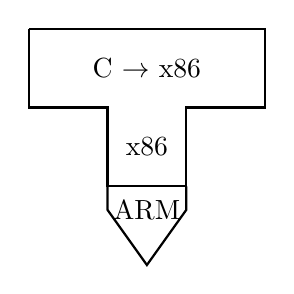
\begin{tikzpicture}
    \draw[thick] (0+1, 0-1) -- (3+1, 0-1)
        -- (3+1, -1-1)
        -- (2+1, -1-1)
        -- (2+1, -2-1)
        -- (1+1, -2-1)
        -- (1+1, -1-1)
        -- (0+1, -1-1)
        -- (0+1, 0-1);
    \node at (1.5+1, -0.5-1) {C $\to$ x86};
    \node at (1.5+1, -1.5-1) {x86};

    \draw[thick] (1+2, 0-3) -- (1+2, -0.3-3)
        -- (0.5+2, -1-3)
        -- (0+2, -0.3-3)
        -- (0+2, 0-3);
    \node at (0.5+2, -0.3-3) {ARM};
    \end{tikzpicture}
\end{figure}
\noindent Similarly, we cannot compile a Java program using a C $\to$ x86 compiler.
\begin{figure}[H]
    \centering
    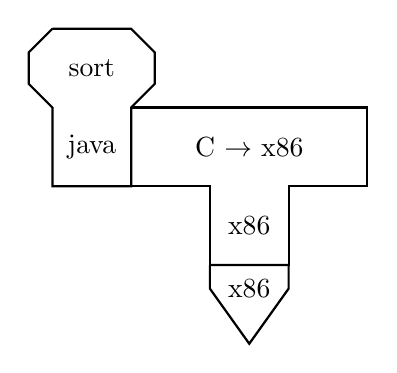
\begin{tikzpicture}
    \draw[thick] (0, 0) -- (1, 0) 
        -- (1.3, -0.3)
        -- (1.3, -0.7)
        -- (1, -1)
        -- (1, -2)
        -- (0, -2)
        -- (0, -1)
        -- (-0.3, -0.7)
        -- (-0.3, -0.3)
        -- (0, 0);
        \node at (0.5, -0.5) {sort};
        \node at (0.5, -1.5) {java};
        
      \draw[thick] (0+1, 0-1) -- (3+1, 0-1)
        -- (3+1, -1-1)
        -- (2+1, -1-1)
        -- (2+1, -2-1)
        -- (1+1, -2-1)
        -- (1+1, -1-1)
        -- (0+1, -1-1)
        -- (0+1, 0-1);
    \node at (1.5+1, -0.5-1) {C $\to$ x86};
    \node at (1.5+1, -1.5-1) {x86};

    \draw[thick] (0+2, 0-3) -- (1+2, 0-3)
        -- (1+2, -0.3-3)
        -- (0.5+2, -1-3)
        -- (0+2, -0.3-3)
        -- (0+2, 0-3);
    \node at (0.5+2, -0.3-3) {x86};
    \end{tikzpicture}
\end{figure}

Now, we will consider representing interpretation via tombstone diagrams. Given an $S$ interpreter expressed in $M$ machine code and a program $P$ expressed in language $S$, we can interpret $P$. This is denoted as follows.
\begin{figure}[H]
    \centering
    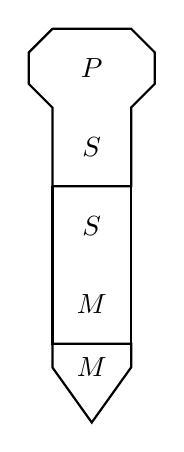
\begin{tikzpicture}
    \draw[thick] (0, 0) -- (1, 0) 
        -- (1.3, -0.3)
        -- (1.3, -0.7)
        -- (1, -1)
        -- (1, -2)
        -- (0, -2)
        -- (0, -1)
        -- (-0.3, -0.7)
        -- (-0.3, -0.3)
        -- (0, 0);
    \node at (0.5, -0.5) {$P$};
    \node at (0.5, -1.5) {$S$};
    
    \draw[thick] (1, -3) -- (1, -2)
        -- (1, -4) 
        -- (0, -4)
        -- (0, -2);
    \node at (0.5, -2.5) {$S$};
    \node at (0.5, -3.5) {$M$};
    
    \draw[thick] (0, 0-4) -- (1, 0-4)
        -- (1, -0.3-4)
        -- (0.5, -1-4)
        -- (0, -0.3-4)
        -- (0, 0-4);
    \node at (0.5, -0.3-4) {$M$};
    \end{tikzpicture}
\end{figure}
\noindent The language in which the program is written (i.e. $S$) must match the language that is being interpreted. Moreover, the language in which the interpreter is written (i.e. $M$) must match the language of the hardware. So, it is possible to interpret a sort program in Ruby with a Ruby interpreter, but not a sort program in C.
\begin{figure}[H]
    \centering
    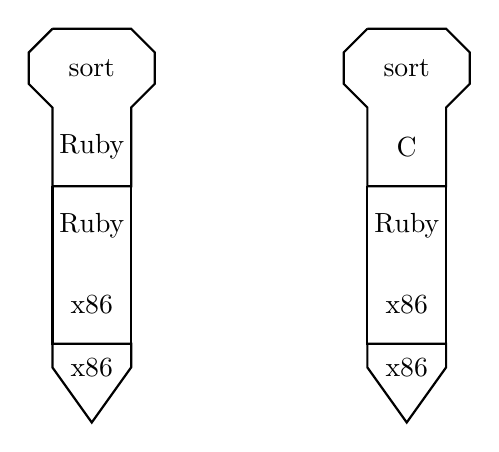
\begin{tikzpicture}
    \draw[thick] (0, 0) -- (1, 0) 
        -- (1.3, -0.3)
        -- (1.3, -0.7)
        -- (1, -1)
        -- (1, -2)
        -- (0, -2)
        -- (0, -1)
        -- (-0.3, -0.7)
        -- (-0.3, -0.3)
        -- (0, 0);
    \node at (0.5, -0.5) {sort};
    \node at (0.5, -1.5) {Ruby};
    
    \draw[thick] (1, -3) -- (1, -2)
        -- (1, -4) 
        -- (0, -4)
        -- (0, -2);
    \node at (0.5, -2.5) {Ruby};
    \node at (0.5, -3.5) {x86};
    
    \draw[thick] (0, 0-4) -- (1, 0-4)
        -- (1, -0.3-4)
        -- (0.5, -1-4)
        -- (0, -0.3-4)
        -- (0, 0-4);
    \node at (0.5, -0.3-4) {x86};

    \draw[thick] (0+4, 0) -- (1+4, 0) 
        -- (1.3+4, -0.3)
        -- (1.3+4, -0.7)
        -- (1+4, -1)
        -- (1+4, -2)
        -- (0+4, -2)
        -- (0+4, -1)
        -- (-0.3+4, -0.7)
        -- (-0.3+4, -0.3)
        -- (0+4, 0);
    \node at (0.5+4, -0.5) {sort};
    \node at (0.5+4, -1.5) {C};
    
    \draw[thick] (1+4, -3) -- (1+4, -2)
        -- (1+4, -4) 
        -- (0+4, -4)
        -- (0+4, -2);
    \node at (0.5+4, -2.5) {Ruby};
    \node at (0.5+4, -3.5) {x86};
    
    \draw[thick] (0+4, 0-4) -- (1+4, 0-4)
        -- (1+4, -0.3-4)
        -- (0.5+4, -1-4)
        -- (0+4, -0.3-4)
        -- (0+4, 0-4);
    \node at (0.5+4, -0.3-4) {x86};
    \end{tikzpicture}
\end{figure}

\subsection{Virtual machines}
A real machine is one whose machine code is executed by hardware. A virtual machine (or an abstract machine) is one whose machine code is executed by an interpreter. We can use tombstone diagrams to denote virtual machines. For example, assume that we designed the architecture and instruction set of a new machine called MVM. Building a hardware prototype would be expensive, and even more to modify.

We can first write an interpreter for MVM machine code (an emulator) expressed in C, for example. This is given below.
\begin{figure}[H]
    \centering
    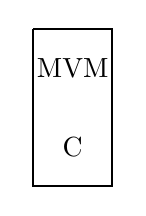
\begin{tikzpicture}
    \draw[thick] (0, 0) -- (1, 0)
        -- (1, -2)
        -- (0, -2)
        -- (0, 0);
    \node at (0.5, -0.5) {MVM};
    \node at (0.5, -1.5) {C};
    \end{tikzpicture}
\end{figure}
\noindent We can then compile it on a real machine, e.g. x86.
\begin{figure}[H]
    \centering
    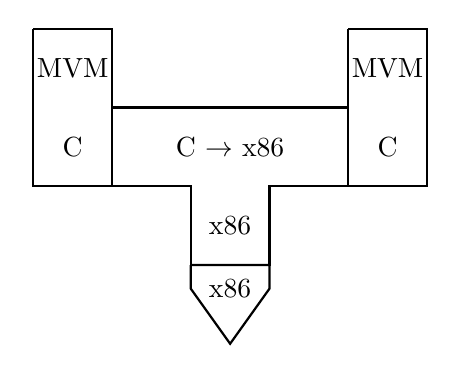
\begin{tikzpicture}
    \draw[thick] (0, 0) -- (1, 0)
        -- (1, -2)
        -- (0, -2)
        -- (0, 0);
    \node at (0.5, -0.5) {MVM};
    \node at (0.5, -1.5) {C};
        
      \draw[thick] (0+1, 0-1) -- (3+1, 0-1)
        -- (3+1, -1-1)
        -- (2+1, -1-1)
        -- (2+1, -2-1)
        -- (1+1, -2-1)
        -- (1+1, -1-1)
        -- (0+1, -1-1)
        -- (0+1, 0-1);
    \node at (1.5+1, -0.5-1) {C $\to$ x86};
    \node at (1.5+1, -1.5-1) {x86};

    \draw[thick] (0+4, 0) -- (1+4, 0)
        -- (1+4, -2)
        -- (0+4, -2)
        -- (0+4, 0);
    \node at (0.5+4, -0.5) {MVM};
    \node at (0.5+4, -1.5) {C};

    \draw[thick] (0+2, 0-3) -- (1+2, 0-3)
        -- (1+2, -0.3-3)
        -- (0.5+2, -1-3)
        -- (0+2, -0.3-3)
        -- (0+2, 0-3);
    \node at (0.5+2, -0.3-3) {x86};
    \end{tikzpicture}
\end{figure}
\noindent Now, we can use the emulator to execute programs $P$ expressed in MVM machine code.
\begin{figure}[H]
    \centering
    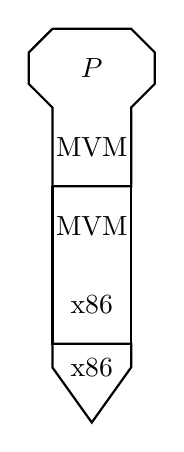
\begin{tikzpicture}
    \draw[thick] (0, 0) -- (1, 0) 
        -- (1.3, -0.3)
        -- (1.3, -0.7)
        -- (1, -1)
        -- (1, -2)
        -- (0, -2)
        -- (0, -1)
        -- (-0.3, -0.7)
        -- (-0.3, -0.3)
        -- (0, 0);
    \node at (0.5, -0.5) {$P$};
    \node at (0.5, -1.5) {MVM};
    
    \draw[thick] (1, -3) -- (1, -2)
        -- (1, -4) 
        -- (0, -4)
        -- (0, -2);
    \node at (0.5, -2.5) {MVM};
    \node at (0.5, -3.5) {x86};
    
    \draw[thick] (0, 0-4) -- (1, 0-4)
        -- (1, -0.3-4)
        -- (0.5, -1-4)
        -- (0, -0.3-4)
        -- (0, 0-4);
    \node at (0.5, -0.3-4) {x86};
    \end{tikzpicture}
\end{figure}
\noindent The bottom two layers are called the MVM virtual machine. This has the same effect as the MVM real machine, given by the following.
\begin{figure}[H]
    \centering
    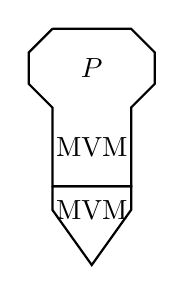
\begin{tikzpicture}
    \draw[thick] (0+4, 0) -- (1+4, 0) 
        -- (1.3+4, -0.3)
        -- (1.3+4, -0.7)
        -- (1+4, -1)
        -- (1+4, -2)
        -- (0+4, -2)
        -- (0+4, -1)
        -- (-0.3+4, -0.7)
        -- (-0.3+4, -0.3)
        -- (0+4, 0);
    \node at (0.5+4, -0.5) {$P$};
    \node at (0.5+4, -1.5) {MVM};
    
    \draw[thick] (0+4, 0-2) -- (1+4, 0-2)
        -- (1+4, -0.3-2)
        -- (0.5+4, -1-2)
        -- (0+4, -0.3-2)
        -- (0+4, 0-2);
    \node at (0.5+4, -0.3-2) {MVM};
    \end{tikzpicture}
\end{figure}
\noindent However, using the MVM real machine would be much faster.

\subsection{Interpretive Compilers}
A compiler takes quite a long time to translate the source program to native machine code, but the subsequent execution is fast. On the other hand, an interpreter starts executing the source program immediately, but the execution is slow. We can combine the two and get an interpretive compiler. It translates the source program into virtual machine (VM) code which is subsequently interpreted.

An interpretive compiler combines fast translation with moderately fast execution, provided that:
\begin{itemize}
    \item the VM code is intermediate-level (lower-level than the source code but higher-level than native machine code);
    \item translation from the source language to VM code is easy and fast;
    \item the VM instructions have simpler formats (so can be analysed quickly by an interpreter).
\end{itemize}

For example, JDK (Java development kit) provides an interpretive compiler for Java. This is based on the JVM (Java virtual machine) that was designed to run Java programs. JVM provides powerful instructions that implement object creation, method calls, array indexing, etc. However, the instructions (called `bytecodes') are similar in format to native machine code, i.e. opcode + operand.

JDK comprises a Java $\to$ JVM compiler and a JVM interpreter. Once JDK has been installed on a real machine, we have the following components:
\begin{figure}[H]
    \centering
    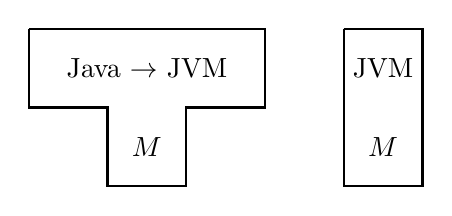
\begin{tikzpicture}
    \draw[thick] (0, 0) -- (3, 0)
        -- (3, -1)
        -- (2, -1)
        -- (2, -2)
        -- (1, -2)
        -- (1, -1)
        -- (0, -1)
        -- (0, 0);
    \node at (1.5, -0.5) {Java $\to$ JVM};
    \node at (1.5, -1.5) {$M$};

    \draw[thick] (0+4, 0) -- (1+4, 0)
        -- (1+4, -2)
        -- (0+4, -2)
        -- (0+4, 0);
    \node at (0.5+4, -0.5) {JVM};
    \node at (0.5+4, -1.5) {$M$};
    \end{tikzpicture}
\end{figure}
\noindent Using these, we can translate Java source program $P$ into JVM code.
\begin{figure}[H]
    \centering
    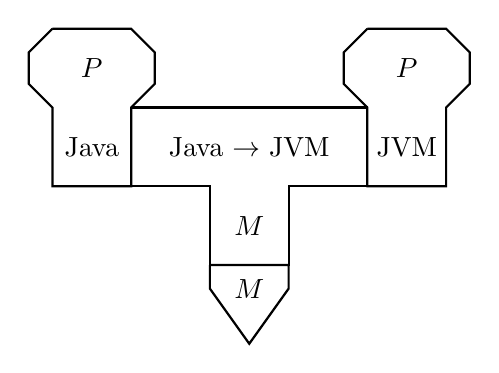
\begin{tikzpicture}
    \draw[thick] (0, 0) -- (1, 0) 
        -- (1.3, -0.3)
        -- (1.3, -0.7)
        -- (1, -1)
        -- (1, -2)
        -- (0, -2)
        -- (0, -1)
        -- (-0.3, -0.7)
        -- (-0.3, -0.3)
        -- (0, 0);
        \node at (0.5, -0.5) {$P$};
        \node at (0.5, -1.5) {Java};
        
      \draw[thick] (0+1, 0-1) -- (3+1, 0-1)
        -- (3+1, -1-1)
        -- (2+1, -1-1)
        -- (2+1, -2-1)
        -- (1+1, -2-1)
        -- (1+1, -1-1)
        -- (0+1, -1-1)
        -- (0+1, 0-1);
    \node at (1.5+1, -0.5-1) {Java $\to$ JVM};
    \node at (1.5+1, -1.5-1) {$M$};

    \draw[thick] (0+4, 0) -- (1+4, 0) 
        -- (1.3+4, -0.3)
        -- (1.3+4, -0.7)
        -- (1+4, -1)
        -- (1+4, -2)
        -- (0+4, -2)
        -- (0+4, -1)
        -- (-0.3+4, -0.7)
        -- (-0.3+4, -0.3)
        -- (0+4, 0);
        \node at (0.5+4, -0.5) {$P$};
        \node at (0.5+4, -1.5) {JVM};

    \draw[thick] (0+2, 0-3) -- (1+2, 0-3)
        -- (1+2, -0.3-3)
        -- (0.5+2, -1-3)
        -- (0+2, -0.3-3)
        -- (0+2, 0-3);
    \node at (0.5+2, -0.3-3) {$M$};
    \end{tikzpicture}
\end{figure}
\noindent Later, the object program is interpreted.
\begin{figure}[H]
    \centering
    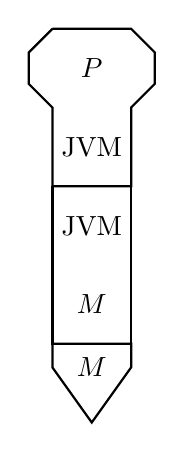
\begin{tikzpicture}
    \draw[thick] (0, 0) -- (1, 0) 
        -- (1.3, -0.3)
        -- (1.3, -0.7)
        -- (1, -1)
        -- (1, -2)
        -- (0, -2)
        -- (0, -1)
        -- (-0.3, -0.7)
        -- (-0.3, -0.3)
        -- (0, 0);
    \node at (0.5, -0.5) {$P$};
    \node at (0.5, -1.5) {JVM};
    
    \draw[thick] (1, -3) -- (1, -2)
        -- (1, -4) 
        -- (0, -4)
        -- (0, -2);
    \node at (0.5, -2.5) {JVM};
    \node at (0.5, -3.5) {$M$};
    
    \draw[thick] (0, 0-4) -- (1, 0-4)
        -- (1, -0.3-4)
        -- (0.5, -1-4)
        -- (0, -0.3-4)
        -- (0, 0-4);
    \node at (0.5, -0.3-4) {$M$};
    \end{tikzpicture}
\end{figure}
\noindent The bottom two tiles are called the Java Virtual Machine.

A just-in-time (JIT) compiler translates virtual machine code to native machine code just prior to execution. More usually, a Java JIT compiler translates JVM code selectively. The interpreter and the JIT compiler work together. The interpreter is instrumented to count method calls. When the interpreter discovers that a method is `hot' (i.e. it is called frequently), it tells the JIT compiler to translate the particular method into native code.

A program is portable if it can be made to run on different machines with minimal change. So, a program $P$ written in Java is portable, but the same program in x86 is not. A compiler that generates native machine code is unportable in that if it must be changed to target a different machine, its code generator must be replaced. However, a compiler that generates suitable virtual machine code can be portable.

So, a portable compiler kit for Java is composed of the following tiles:
\begin{figure}[H]
    \centering
    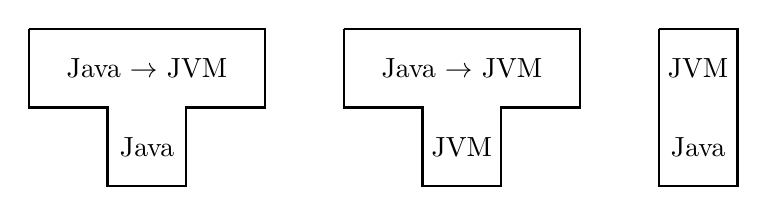
\begin{tikzpicture}
    \draw[thick] (0, 0) -- (3, 0)
        -- (3, -1)
        -- (2, -1)
        -- (2, -2)
        -- (1, -2)
        -- (1, -1)
        -- (0, -1)
        -- (0, 0);
    \node at (1.5, -0.5) {Java $\to$ JVM};
    \node at (1.5, -1.5) {Java};
    
    \draw[thick] (0+4, 0) -- (3+4, 0)
        -- (3+4, -1)
        -- (2+4, -1)
        -- (2+4, -2)
        -- (1+4, -2)
        -- (1+4, -1)
        -- (0+4, -1)
        -- (0+4, 0);
    \node at (1.5+4, -0.5) {Java $\to$ JVM};
    \node at (1.5+4, -1.5) {JVM};

    \draw[thick] (0+8, 0) -- (1+8, 0)
        -- (1+8, -2)
        -- (0+8, -2)
        -- (0+8, 0);
    \node at (0.5+8, -0.5) {JVM};
    \node at (0.5+8, -1.5) {Java};
    \end{tikzpicture}
\end{figure}
\noindent We can install this kit on machine $M$. But, we cannot run the JVM interpreter until we have a running Java compiler. Similarly, we cannot run the Java compiler until we have a running JVM interpreter.

To progress, we first rewrite the JVM interpreter, e.g. in C.
\begin{figure}[H]
    \centering
    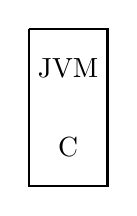
\begin{tikzpicture}
    \draw[thick] (0+8, 0) -- (1+8, 0)
        -- (1+8, -2)
        -- (0+8, -2)
        -- (0+8, 0);
    \node at (0.5+8, -0.5) {JVM};
    \node at (0.5+8, -1.5) {C};
    \end{tikzpicture}
\end{figure}
\noindent Then, we compile the JVM interpreter on $M$.
\begin{figure}[H]
    \centering
    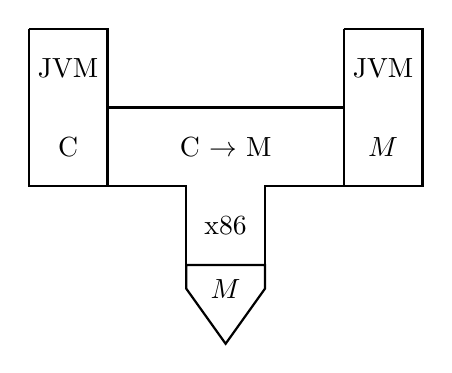
\begin{tikzpicture}
    \draw[thick] (0, 0) -- (1, 0)
        -- (1, -2)
        -- (0, -2)
        -- (0, 0);
    \node at (0.5, -0.5) {JVM};
    \node at (0.5, -1.5) {C};
        
      \draw[thick] (0+1, 0-1) -- (3+1, 0-1)
        -- (3+1, -1-1)
        -- (2+1, -1-1)
        -- (2+1, -2-1)
        -- (1+1, -2-1)
        -- (1+1, -1-1)
        -- (0+1, -1-1)
        -- (0+1, 0-1);
    \node at (1.5+1, -0.5-1) {C $\to$ M};
    \node at (1.5+1, -1.5-1) {x86};

    \draw[thick] (0+4, 0) -- (1+4, 0)
        -- (1+4, -2)
        -- (0+4, -2)
        -- (0+4, 0);
    \node at (0.5+4, -0.5) {JVM};
    \node at (0.5+4, -1.5) {$M$};

    \draw[thick] (0+2, 0-3) -- (1+2, 0-3)
        -- (1+2, -0.3-3)
        -- (0.5+2, -1-3)
        -- (0+2, -0.3-3)
        -- (0+2, 0-3);
    \node at (0.5+2, -0.3-3) {$M$};
    \end{tikzpicture}
\end{figure}
\noindent Now, we have an interpretive compiler. But, the compiler itself must be interpreted in this case.
\begin{figure}[H]
    \centering
    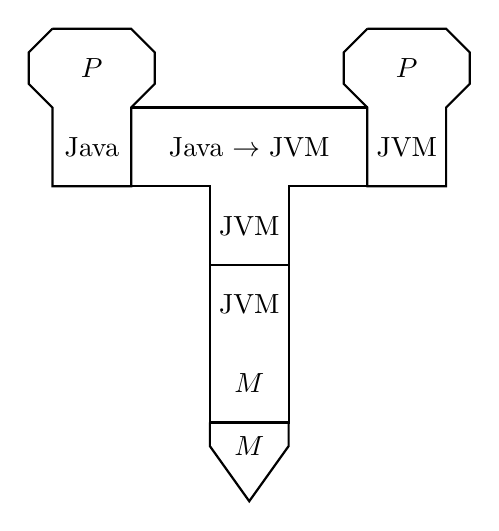
\begin{tikzpicture}
    \draw[thick] (0, 0) -- (1, 0) 
        -- (1.3, -0.3)
        -- (1.3, -0.7)
        -- (1, -1)
        -- (1, -2)
        -- (0, -2)
        -- (0, -1)
        -- (-0.3, -0.7)
        -- (-0.3, -0.3)
        -- (0, 0);
        \node at (0.5, -0.5) {$P$};
        \node at (0.5, -1.5) {Java};
        
      \draw[thick] (0+1, 0-1) -- (3+1, 0-1)
        -- (3+1, -1-1)
        -- (2+1, -1-1)
        -- (2+1, -2-1)
        -- (1+1, -2-1)
        -- (1+1, -1-1)
        -- (0+1, -1-1)
        -- (0+1, 0-1);
    \node at (1.5+1, -0.5-1) {Java $\to$ JVM};
    \node at (1.5+1, -1.5-1) {JVM};

    \draw[thick] (0+4, 0) -- (1+4, 0) 
        -- (1.3+4, -0.3)
        -- (1.3+4, -0.7)
        -- (1+4, -1)
        -- (1+4, -2)
        -- (0+4, -2)
        -- (0+4, -1)
        -- (-0.3+4, -0.7)
        -- (-0.3+4, -0.3)
        -- (0+4, 0);
    \node at (0.5+4, -0.5) {$P$};
    \node at (0.5+4, -1.5) {JVM};
    
    \draw[thick] (0+2, 0-3) -- (1+2, 0-3)
        -- (1+2, -2-3)
        -- (0+2, -2-3)
        -- (0+2, 0-3);
    \node at (0.5+2, -0.5-3) {JVM};
    \node at (0.5+2, -1.5-3) {$M$};

    \draw[thick] (0+2, 0-5) -- (1+2, 0-5)
        -- (1+2, -0.3-5)
        -- (0.5+2, -1-5)
        -- (0+2, -0.3-5)
        -- (0+2, 0-5);
    \node at (0.5+2, -0.3-5) {$M$};
    \end{tikzpicture}
\end{figure}
\noindent Using the result, we can interpret the program $P$ using the JVM.
\begin{figure}[H]
    \centering
    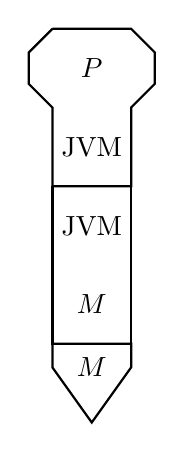
\begin{tikzpicture}
    \draw[thick] (0, 0) -- (1, 0) 
        -- (1.3, -0.3)
        -- (1.3, -0.7)
        -- (1, -1)
        -- (1, -2)
        -- (0, -2)
        -- (0, -1)
        -- (-0.3, -0.7)
        -- (-0.3, -0.3)
        -- (0, 0);
    \node at (0.5, -0.5) {$P$};
    \node at (0.5, -1.5) {JVM};
    
    \draw[thick] (1, -3) -- (1, -2)
        -- (1, -4) 
        -- (0, -4)
        -- (0, -2);
    \node at (0.5, -2.5) {JVM};
    \node at (0.5, -3.5) {$M$};
    
    \draw[thick] (0, 0-4) -- (1, 0-4)
        -- (1, -0.3-4)
        -- (0.5, -1-4)
        -- (0, -0.3-4)
        -- (0, 0-4);
    \node at (0.5, -0.3-4) {$M$};
    \end{tikzpicture}
\end{figure}
\noindent Here, the compilation stage is very slow, but it can be improved by bootstraping.

Assume that we have an $S \to T$ translator expressed in language $S$.
\begin{figure}[H]
    \centering
    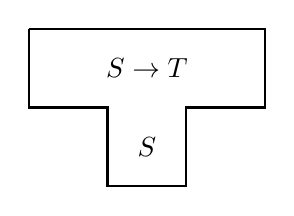
\begin{tikzpicture}
    \draw[thick] (0, 0) -- (3, 0)
        -- (3, -1)
        -- (2, -1)
        -- (2, -2)
        -- (1, -2)
        -- (1, -1)
        -- (0, -1)
        -- (0, 0);
    \node at (1.5, -0.5) {$S \to T$};
    \node at (1.5, -1.5) {$S$};
    \end{tikzpicture}
\end{figure}
\noindent We can use this translator to translate itself. This process is called bootstraping. It is a useful tool for improving an existing compiler. This is because it makes the compilation process faster, which makes it generate faster object code. We can bootstrap a portable compiler to make a true compiler, by translating virtual machine code into native machine code.

For example, consider the Java portable compiler kit.
\begin{figure}[H]
    \centering
    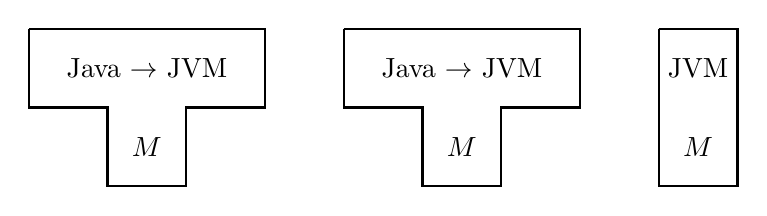
\begin{tikzpicture}
    \draw[thick] (0, 0) -- (3, 0)
        -- (3, -1)
        -- (2, -1)
        -- (2, -2)
        -- (1, -2)
        -- (1, -1)
        -- (0, -1)
        -- (0, 0);
    \node at (1.5, -0.5) {Java $\to$ JVM};
    \node at (1.5, -1.5) {$M$};
    
    \draw[thick] (0+4, 0) -- (3+4, 0)
        -- (3+4, -1)
        -- (2+4, -1)
        -- (2+4, -2)
        -- (1+4, -2)
        -- (1+4, -1)
        -- (0+4, -1)
        -- (0+4, 0);
    \node at (1.5+4, -0.5) {Java $\to$ JVM};
    \node at (1.5+4, -1.5) {$M$};

    \draw[thick] (0+8, 0) -- (1+8, 0)
        -- (1+8, -2)
        -- (0+8, -2)
        -- (0+8, 0);
    \node at (0.5+8, -0.5) {JVM};
    \node at (0.5+8, -1.5) {$M$};
    \end{tikzpicture}
\end{figure}
\noindent We also constructed a JVM interpreter in machine language $M$.
\begin{figure}[H]
    \centering
    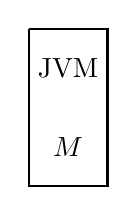
\begin{tikzpicture}
    \draw[thick] (0+8, 0) -- (1+8, 0)
        -- (1+8, -2)
        -- (0+8, -2)
        -- (0+8, 0);
    \node at (0.5+8, -0.5) {JVM};
    \node at (0.5+8, -1.5) {$M$};
    \end{tikzpicture}
\end{figure}
\noindent We can write a JVM $\to$ M translator in Java itself. We then compile it into JVM using the existing, slow compiler.
\begin{figure}[H]
    \centering
    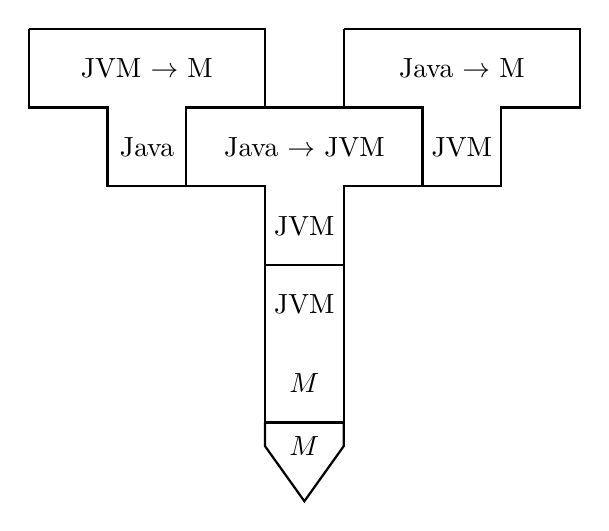
\begin{tikzpicture}
    \draw[thick] (0-1, 0) -- (3-1, 0)
        -- (3-1, -1)
        -- (2-1, -1)
        -- (2-1, -2)
        -- (1-1, -2)
        -- (1-1, -1)
        -- (0-1, -1)
        -- (0-1, 0);
    \node at (1.5-1, -0.5) {JVM $\to$ M};
    \node at (1.5-1, -1.5) {Java};
        
      \draw[thick] (0+1, 0-1) -- (3+1, 0-1)
        -- (3+1, -1-1)
        -- (2+1, -1-1)
        -- (2+1, -2-1)
        -- (1+1, -2-1)
        -- (1+1, -1-1)
        -- (0+1, -1-1)
        -- (0+1, 0-1);
    \node at (1.5+1, -0.5-1) {Java $\to$ JVM};
    \node at (1.5+1, -1.5-1) {JVM};

    \draw[thick] (0+3, 0) -- (3+3, 0)
        -- (3+3, -1)
        -- (2+3, -1)
        -- (2+3, -2)
        -- (1+3, -2)
        -- (1+3, -1)
        -- (0+3, -1)
        -- (0+3, 0);
    \node at (1.5+3, -0.5) {Java $\to$ M};
    \node at (1.5+3, -1.5) {JVM};

    \draw[thick] (1+2, -3-1) -- (1+2, -2-1)
        -- (1+2, -4-1) 
        -- (0+2, -4-1)
        -- (0+2, -2-1);
    \node at (0.5+2, -2.5-1) {JVM};
    \node at (0.5+2, -3.5-1) {$M$};

    \draw[thick] (0+2, 0-5) -- (1+2, 0-5)
        -- (1+2, -0.3-5)
        -- (0.5+2, -1-5)
        -- (0+2, -0.3-5)
        -- (0+2, 0-5);
    \node at (0.5+2, -0.3-5) {$M$};
    \end{tikzpicture}
\end{figure}
\noindent Next, we can use this JVM $\to$ M translator to translate itself.
\begin{figure}[H]
    \centering
    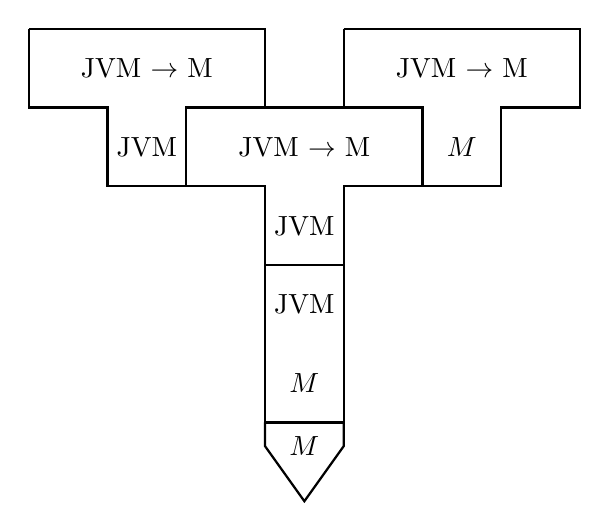
\begin{tikzpicture}
    \draw[thick] (0-1, 0) -- (3-1, 0)
        -- (3-1, -1)
        -- (2-1, -1)
        -- (2-1, -2)
        -- (1-1, -2)
        -- (1-1, -1)
        -- (0-1, -1)
        -- (0-1, 0);
    \node at (1.5-1, -0.5) {JVM $\to$ M};
    \node at (1.5-1, -1.5) {JVM};
        
      \draw[thick] (0+1, 0-1) -- (3+1, 0-1)
        -- (3+1, -1-1)
        -- (2+1, -1-1)
        -- (2+1, -2-1)
        -- (1+1, -2-1)
        -- (1+1, -1-1)
        -- (0+1, -1-1)
        -- (0+1, 0-1);
    \node at (1.5+1, -0.5-1) {JVM $\to$ M};
    \node at (1.5+1, -1.5-1) {JVM};

    \draw[thick] (0+3, 0) -- (3+3, 0)
        -- (3+3, -1)
        -- (2+3, -1)
        -- (2+3, -2)
        -- (1+3, -2)
        -- (1+3, -1)
        -- (0+3, -1)
        -- (0+3, 0);
    \node at (1.5+3, -0.5) {JVM $\to$ M};
    \node at (1.5+3, -1.5) {$M$};

    \draw[thick] (1+2, -3-1) -- (1+2, -2-1)
        -- (1+2, -4-1) 
        -- (0+2, -4-1)
        -- (0+2, -2-1);
    \node at (0.5+2, -2.5-1) {JVM};
    \node at (0.5+2, -3.5-1) {$M$};

    \draw[thick] (0+2, 0-5) -- (1+2, 0-5)
        -- (1+2, -0.3-5)
        -- (0.5+2, -1-5)
        -- (0+2, -0.3-5)
        -- (0+2, 0-5);
    \node at (0.5+2, -0.3-5) {$M$};
    \end{tikzpicture}
\end{figure}
\noindent This is the actual bootstrap. It generates the JVM $\to$ M translator, expressed in $M$ machine code. Finally, we can translate the Java $\to$ JVM compiler into $M$ machine code.
\begin{figure}[H]
    \centering
    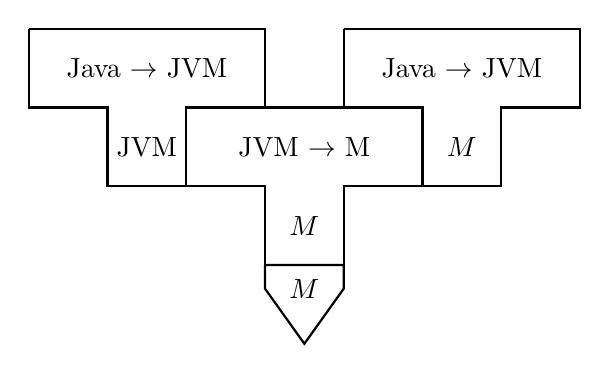
\begin{tikzpicture}
    \draw[thick] (0-1, 0) -- (3-1, 0)
        -- (3-1, -1)
        -- (2-1, -1)
        -- (2-1, -2)
        -- (1-1, -2)
        -- (1-1, -1)
        -- (0-1, -1)
        -- (0-1, 0);
    \node at (1.5-1, -0.5) {Java $\to$ JVM};
    \node at (1.5-1, -1.5) {JVM};
        
      \draw[thick] (0+1, 0-1) -- (3+1, 0-1)
        -- (3+1, -1-1)
        -- (2+1, -1-1)
        -- (2+1, -2-1)
        -- (1+1, -2-1)
        -- (1+1, -1-1)
        -- (0+1, -1-1)
        -- (0+1, 0-1);
    \node at (1.5+1, -0.5-1) {JVM $\to$ M};
    \node at (1.5+1, -1.5-1) {$M$};

    \draw[thick] (0+3, 0) -- (3+3, 0)
        -- (3+3, -1)
        -- (2+3, -1)
        -- (2+3, -2)
        -- (1+3, -2)
        -- (1+3, -1)
        -- (0+3, -1)
        -- (0+3, 0);
    \node at (1.5+3, -0.5) {Java $\to$ JVM};
    \node at (1.5+3, -1.5) {$M$};

    \draw[thick] (0+2, 0-3) -- (1+2, 0-3)
        -- (1+2, -0.3-3)
        -- (0.5+2, -1-3)
        -- (0+2, -0.3-3)
        -- (0+2, 0-3);
    \node at (0.5+2, -0.3-3) {$M$};
    \end{tikzpicture}
\end{figure}

Now, we have a 2-stage Java $\to$ M compiler.
\begin{figure}[H]
    \centering
    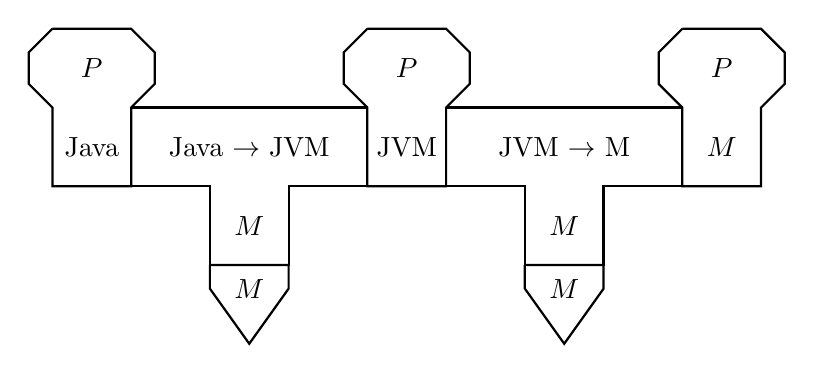
\begin{tikzpicture}
    \draw[thick] (0, 0) -- (1, 0) 
        -- (1.3, -0.3)
        -- (1.3, -0.7)
        -- (1, -1)
        -- (1, -2)
        -- (0, -2)
        -- (0, -1)
        -- (-0.3, -0.7)
        -- (-0.3, -0.3)
        -- (0, 0);
        \node at (0.5, -0.5) {$P$};
        \node at (0.5, -1.5) {Java};
        
      \draw[thick] (0+1, 0-1) -- (3+1, 0-1)
        -- (3+1, -1-1)
        -- (2+1, -1-1)
        -- (2+1, -2-1)
        -- (1+1, -2-1)
        -- (1+1, -1-1)
        -- (0+1, -1-1)
        -- (0+1, 0-1);
    \node at (1.5+1, -0.5-1) {Java $\to$ JVM};
    \node at (1.5+1, -1.5-1) {$M$};

    \draw[thick] (0+4, 0) -- (1+4, 0) 
        -- (1.3+4, -0.3)
        -- (1.3+4, -0.7)
        -- (1+4, -1)
        -- (1+4, -2)
        -- (0+4, -2)
        -- (0+4, -1)
        -- (-0.3+4, -0.7)
        -- (-0.3+4, -0.3)
        -- (0+4, 0);
        \node at (0.5+4, -0.5) {$P$};
        \node at (0.5+4, -1.5) {JVM};

    \draw[thick] (0+2, 0-3) -- (1+2, 0-3)
        -- (1+2, -0.3-3)
        -- (0.5+2, -1-3)
        -- (0+2, -0.3-3)
        -- (0+2, 0-3);
    \node at (0.5+2, -0.3-3) {$M$};
        
     \draw[thick] (0+5, 0-1) -- (3+5, 0-1)
        -- (3+5, -1-1)
        -- (2+5, -1-1)
        -- (2+5, -2-1)
        -- (1+5, -2-1)
        -- (1+5, -1-1)
        -- (0+5, -1-1)
        -- (0+5, 0-1);
    \node at (1.5+5, -0.5-1) {JVM $\to$ M};
    \node at (1.5+5, -1.5-1) {$M$};

    \draw[thick] (0+8, 0) -- (1+8, 0) 
        -- (1.3+8, -0.3)
        -- (1.3+8, -0.7)
        -- (1+8, -1)
        -- (1+8, -2)
        -- (0+8, -2)
        -- (0+8, -1)
        -- (-0.3+8, -0.7)
        -- (-0.3+8, -0.3)
        -- (0+8, 0);
        \node at (0.5+8, -0.5) {$P$};
        \node at (0.5+8, -1.5) {$M$};

    \draw[thick] (0+6, 0-3) -- (1+6, 0-3)
        -- (1+6, -0.3-3)
        -- (0.5+6, -1-3)
        -- (0+6, -0.3-3)
        -- (0+6, 0-3);
    \node at (0.5+6, -0.3-3) {$M$};
    \end{tikzpicture}
\end{figure}
\noindent This Java compiler is improved in two respects. It compilers faster since it is expressed in native machine code. It also generates faster object code.

\newpage

\section{Interpretation}
An $S$ interpreter accepts code expressed in language $S$ and immediately executes that code. Assuming that the code to be interpreted is just a sequence of simple instructions (with conditional and unconditional jumps), the interpreter:
\begin{itemize}
    \item first initialises the state,
    \item then repeatedly fetches, analyses and executes the next instruction, and
    \item updates the state as an instruction gets updated, as required.
\end{itemize}

Virtual machine code typically consists of:
\begin{itemize}
    \item load and store instructions,
    \item arithmetic and logical instructions,
    \item conditional and unconditional jumps, 
    \item call and return instructions, etc.
\end{itemize}
The virtual machine state typically consists of storage (code and data) along with registers (status, program counter, stack pointer, etc.).

\subsection{SVM}
Simple Virtual Machine (SVM) is suitable for executing programs in simple imperative PLs. Consider we have the following source code in a C-style language:
\begin{lstlisting}[language=java]
p = 1;
while (p < n) {
    p = 10 * p;
}
\end{lstlisting}
The corresponding SVM code for it is the following:
\begin{lstlisting}[language=SVM]
// load constant 1
LOADC 1
// store the constant 1 at address 2 (variable p)
STOREG 2
// load from address 2 (variable p)
LOADG 2
// load from address 1 (variable n)
LOADG 1
// compare p < n
COMPLT
// if false, jump to 29 = line 24 (and halt)
JUMPF 29
// load constant 10
LOADC 10
// load from address 2 (variable p)
LOADG 2
// multiply p and 10
MUL
// store p*10 to address 2
STOREG 2
// jump to 6 = line 6
JUMP 6
// halt
HALT
\end{lstlisting}

The SVM storage is composed of the code store and the data store. The code store is a fixed array of bytes (32 768 bytes) providing space for instructions. The data store is a fixed array of words (32 768 bytes) providing a stack to contain global and local data. The main registers for SVM are:
\begin{itemize}
    \item \texttt{pc} (program counter) points to the next instruction to be executed
    \item \texttt{sp} (stack pointer) points to the top of the stack
    \item \texttt{fp} (frame pointer) points to the base of the topmost frame
    \item \texttt{status} indicates whether the program is running, failed or halted.
\end{itemize}

The following image illustrates the code store of the SVM code above.
\begin{figure}[H]
    \centering
    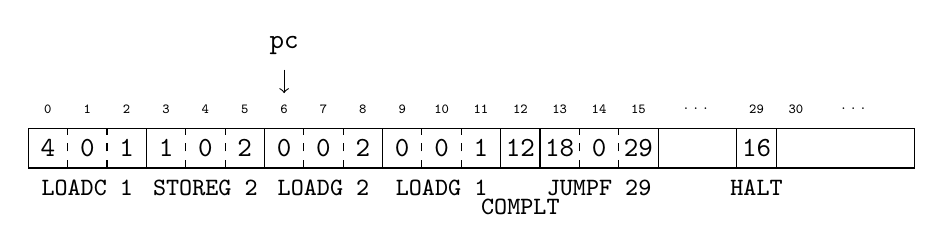
\begin{tikzpicture}
    \node at (0, 1) {\tiny\texttt{0}};
    \node at (0, 0.5) {\texttt{4}};
    \foreach \x[count=\i] in {0, 1, 1, 0, 2, 0, 0, 2, 0, 0, 1, 12, 18, 0, 29} {
        \node at (\i*0.5, 1) {\tiny\texttt{\i}};
        \node at (\i*0.5, 0.5) {\texttt{\x}};
    }
    \draw (-0.25, 0.25) -- (-0.25, 0.75) -- (11, 0.75) -- (11, 0.25) -- cycle;
    \foreach \i in {1, 2, 4, 5, 7, 8, 10, 11, 14, 15} {
        \draw[dashed] (\i*0.5-0.25, 0.25) -- (\i*0.5-0.25, 0.75);
    }
     \foreach \i in {3, 6, 9, 12, 13, 16, 18, 19} {
        \draw (\i*0.5-0.25, 0.25) -- (\i*0.5-0.25, 0.75);
    }
    \node at (8.25, 1) {\tiny$\dots$};
    
    \node at (9, 1) {\tiny\texttt{29}};
    \node at (9, 0.5) {\texttt{16}};

    \node at (9.5, 1) {\tiny\texttt{30}};
    \node at (10.25, 1) {\tiny$\dots$};
    
    \foreach \x[count=\i] in {LOADC 1, STOREG 2, LOADG 2, LOADG 1} {
        \node at (\i*1.5-1, 0) {\small\texttt{\x}};
    }
    \node at (6, -.25) {\small\texttt{COMPLT}};
    \node at (7, 0) {\small\texttt{JUMPF 29}};
    
    \node at (9, 0) {\small\texttt{HALT}};
    
    \draw[->] (3, 1.5) -- (3, 1.2);
    \node at (3, 1.8) {\texttt{pc}};
    
    \end{tikzpicture}
    \caption{An illustration of the code source.}
\end{figure}
\noindent Each instruction occupies 1, 2 or 3 bytes, e.g. \texttt{STOREG 2} occupies 3 bytes, while \texttt{COMPLT} occupies only 1. The register \texttt{pc} is pointing to 6, meaning that is the next instruction to be executed. The final part (after \texttt{30}) is the unused part of the code source.

Next, the following figure illustrates the data store.
\begin{figure}[H]
    \centering
    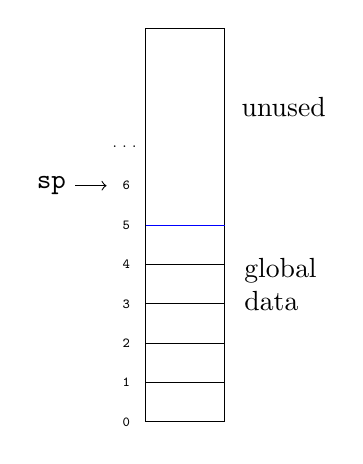
\begin{tikzpicture}
    \draw (0, 0) -- (1, 0)
        -- (1, 5)
        -- (0, 5)
        -- cycle;
    
    \foreach \i in {0, 1, ..., 5} {
        \node at (-0.25, \i*0.5) {\tiny\texttt{\i}};
        \draw (0, \i*0.5) -- (1, \i*0.5);
    }
    \node at (-0.25, 3) {\tiny\texttt{6}};
    \node at (-0.25, 3.5) {\tiny$\dots$};
    
    
    \node at (1.75, 4) {unused};
    \node[text width=1cm] at (1.75, 1.75) {global data};
    
    \draw[blue] (0, 2.5) -- (1, 2.5);
    
    \draw[->] (-.9, 3) -- (-.5, 3);
    \node at (-1.2, 3) {\texttt{sp}};
    \end{tikzpicture}
    \caption{An illustration of the data store at the start.}
\end{figure}
\noindent The register \texttt{sp} is pointing to 6, meaning that all the positions above 6 (including it) is unused and empty. At the bottom, there is only global data on the stack. As the program executes, we load further data, so we might end up at the following state.
\begin{figure}[H]
    \centering
    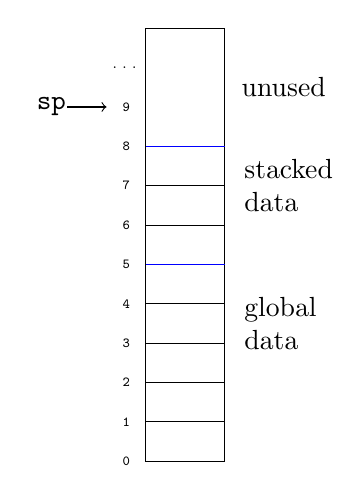
\begin{tikzpicture}
    \draw (0, 0) -- (1, 0)
        -- (1, 5.5)
        -- (0, 5.5)
        -- cycle;
    
    \foreach \i in {0, 1, ..., 8} {
        \node at (-0.25, \i*0.5) {\tiny\texttt{\i}};
        \draw (0, \i*0.5) -- (1, \i*0.5);
    }
    \draw[blue] (0, 2.5) -- (1, 2.5);
    \draw[blue] (0, 4) -- (1, 4);
    
    \node at (-0.25, 4.5) {\tiny\texttt{9}};
    \node at (-0.25, 5) {\tiny$\dots$};
    
    \node[text width=1cm] at (1.75, 3.5) {stacked data};
    \node[text width=1cm] at (1.75, 1.75) {global data};
    \node at (1.75, 4.75) {unused};
    
    \draw[->] (-1, 4.5) -- (-.5, 4.5);
    \node at (-1.2, 4.5) {\texttt{sp}};
    \end{tikzpicture}
    \caption{An illustration of the data store during execution.}
\end{figure}

The following is a simplified version of the SVM instruction set.
\begin{table}[H]
    \centering
    \begin{tabular}{|c|c|c|}
        \hline
        Opcode & Mnemonic & Behavior \\
        \hline
        6 & \texttt{ADD} & pop $w_2$; pop $w_1$; push $(w_1 + w_2)$ \\
        7 & \texttt{SUB} & pop $w_2$; pop $w_1$; push $(w_1 - w_2)$ \\
        8 & \texttt{MUL} & pop $w_2$; pop $w_1$; push $(w_1 * w_2)$ \\
        9 & \texttt{DOV} & pop $w_2$; pop $w_1$; push $(w_1 / w_2)$ \\
        10 & \texttt{CMPEQ} & pop $w_2$; pop $w_1$; push (if $w_1 = w_2$ then 1 else 0) \\
        11 & \texttt{CMPLT} & pop $w_2$; pop $w_1$; push (if $w_1 < w_2$ then 1 else 0) \\
        14 & \texttt{INV} & pop $w$; push (if $w=0$ then 1 else 0) \\
        0 & \texttt{LOADG d} & $w$ $\leftarrow$ word at address $d$; push $w$ \\
        1 & \texttt{STOREG d} & pop $w$; word at address $d$ $\leftarrow$ $w$ \\
        4 & \texttt{LOADC v} & push $v$ \\
        16 & \texttt{HALT}  & status $\leftarrow$ halted \\
        17 & \texttt{JUMP c} & pc $\leftarrow$ c \\
        18 & \texttt{JUMPF c} & pop w; if $w = 0$ then pc $\leftarrow$ c \\
        19 & \texttt{JUMPT c} & pop w; if $w \neq 0$ then pc $\leftarrow$ c \\
        \hline
    \end{tabular}
    \caption{The SVM Instruction Set}
\end{table}

We will illustrate how the data store changes as we execute the program. So, consider we are evaluating the following expression: \texttt{(7 + 3)*(5 - 2)}. In SVM, it is the following:
\begin{lstlisting}[language=SVM]
// load constant 7
LOADC 7
// load constant 3
LOADC 3
// add 7 and 3 = 10
ADD
// load constant 3
LOADC 5
// load constant 2
LOADC 2
// subtract 2 from 5 = 3
SUB
// multiply 10 and 3 = 30
MUL
\end{lstlisting}
We will illustrate the execution with the data store. Assume that the initial state of the stack is the following.
\begin{figure}[H]
    \centering
    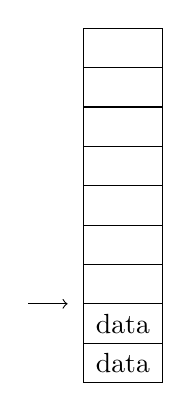
\begin{tikzpicture}
    \draw (0, 0) -- (1, 0)
        -- (1, 4.5)
        -- (0, 4.5)
        -- cycle;
    
    \foreach \i in {0, 1, ..., 8} {
        \draw (0, \i*0.5) -- (1, \i*0.5);
    }
    
    \foreach \x[count=\i] in {data, data} {
        \node at (0.5, 0.5*\i-0.25) {\x};
    }
    
    \draw[->] (-.7, 1) -- (-.2, 1);
    \end{tikzpicture}
\end{figure}
\noindent The arrow denotes the stack pointer \texttt{sp}. We first execute \texttt{LOADC 7}, which will add 7 to the stack.
\begin{figure}[H]
    \centering
    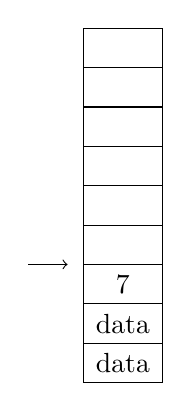
\begin{tikzpicture}
    \draw (0, 0) -- (1, 0)
        -- (1, 4.5)
        -- (0, 4.5)
        -- cycle;
    
    \foreach \i in {0, 1, ..., 8} {
        \draw (0, \i*0.5) -- (1, \i*0.5);
    }
    
    \foreach \x[count=\i] in {data, data, 7} {
        \node at (0.5, 0.5*\i-0.25) {\x};
    }
    
    \draw[->] (-.7, 1.5) -- (-.2, 1.5);
    \end{tikzpicture}
\end{figure}
\noindent Next, we execute \texttt{LOADC 3}, which will add 3 to the stack.
\begin{figure}[H]
    \centering
    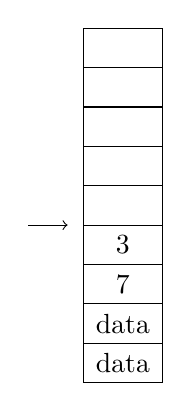
\begin{tikzpicture}
    \draw (0, 0) -- (1, 0)
        -- (1, 4.5)
        -- (0, 4.5)
        -- cycle;
    
    \foreach \i in {0, 1, ..., 8} {
        \draw (0, \i*0.5) -- (1, \i*0.5);
    }
    
    \foreach \x[count=\i] in {data, data, 7, 3} {
        \node at (0.5, 0.5*\i-0.25) {\x};
    }
    
    \draw[->] (-.7, 2) -- (-.2, 2);
    \end{tikzpicture}
\end{figure}
\noindent The next command is \texttt{ADD}. By its specification, we pop $w_2 = 3$ and $w_1 = 7$, and push $w_1 + w_2 = 10$.
\begin{figure}[H]
    \centering
    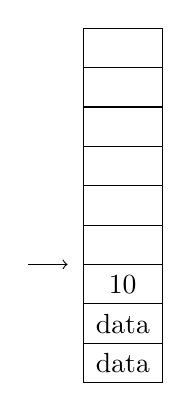
\begin{tikzpicture}
    \draw (0, 0) -- (1, 0)
        -- (1, 4.5)
        -- (0, 4.5)
        -- cycle;
    
    \foreach \i in {0, 1, ..., 8} {
        \draw (0, \i*0.5) -- (1, \i*0.5);
    }
    
    \foreach \x[count=\i] in {data, data, 10} {
        \node at (0.5, 0.5*\i-0.25) {\x};
    }
    
    \draw[->] (-.7, 1.5) -- (-.2, 1.5);
    \end{tikzpicture}
\end{figure}
\noindent The next command is \texttt{LOADC 5}. So, we push 5 to the stack.
\begin{figure}[H]
    \centering
    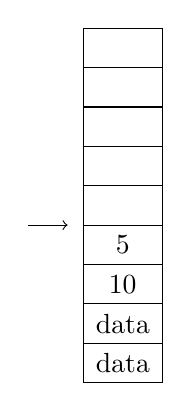
\begin{tikzpicture}
    \draw (0, 0) -- (1, 0)
        -- (1, 4.5)
        -- (0, 4.5)
        -- cycle;
    
    \foreach \i in {0, 1, ..., 8} {
        \draw (0, \i*0.5) -- (1, \i*0.5);
    }
    
    \foreach \x[count=\i] in {data, data, 10, 5} {
        \node at (0.5, 0.5*\i-0.25) {\x};
    }
    
    \draw[->] (-.7, 2) -- (-.2, 2);
    \end{tikzpicture}
\end{figure}
\noindent Now, we perform \texttt{LOADC 2}, when we push 2 to the stack.
\begin{figure}[H]
    \centering
    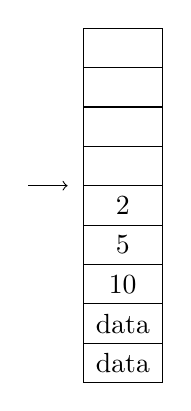
\begin{tikzpicture}
    \draw (0, 0) -- (1, 0)
        -- (1, 4.5)
        -- (0, 4.5)
        -- cycle;
    
    \foreach \i in {0, 1, ..., 8} {
        \draw (0, \i*0.5) -- (1, \i*0.5);
    }
    
    \foreach \x[count=\i] in {data, data, 10, 5, 2} {
        \node at (0.5, 0.5*\i-0.25) {\x};
    }
    
    \draw[->] (-.7, 2.5) -- (-.2, 2.5);
    \end{tikzpicture}
\end{figure}
\noindent The next command is \texttt{SUB}. So, we pop $w_2 = 2$ and $w_1 = 5$, and push $w_1 - w_2 = 3$.
\begin{figure}[H]
    \centering
    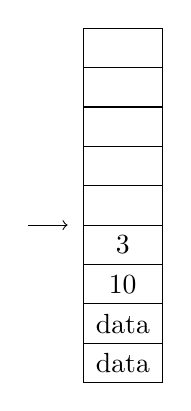
\begin{tikzpicture}
    \draw (0, 0) -- (1, 0)
        -- (1, 4.5)
        -- (0, 4.5)
        -- cycle;
    
    \foreach \i in {0, 1, ..., 8} {
        \draw (0, \i*0.5) -- (1, \i*0.5);
    }
    
    \foreach \x[count=\i] in {data, data, 10, 3} {
        \node at (0.5, 0.5*\i-0.25) {\x};
    }
    
    \draw[->] (-.7, 2) -- (-.2, 2);
    \end{tikzpicture}
\end{figure}
\noindent The final command is \texttt{MUL}. So, we pop $w_2 = 3$ and $w_1 = 10$, and push $w_1 * w_2 = 30$.
\begin{figure}[H]
    \centering
    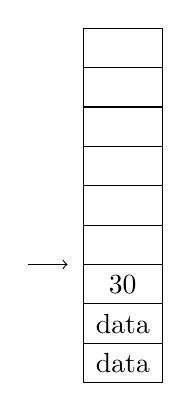
\begin{tikzpicture}
    \draw (0, 0) -- (1, 0)
        -- (1, 4.5)
        -- (0, 4.5)
        -- cycle;
    
    \foreach \i in {0, 1, ..., 8} {
        \draw (0, \i*0.5) -- (1, \i*0.5);
    }
    
    \foreach \x[count=\i] in {data, data, 30} {
        \node at (0.5, 0.5*\i-0.25) {\x};
    }
    
    \draw[->] (-.7, 1.5) -- (-.2, 1.5);
    \end{tikzpicture}
\end{figure}

\subsection{Writing interpreters}
Interpreters are commonly written in C or Java. In such an interpreter, the virtual machine state is represented by a group of variables. Each instruction is executed by inspecting and/or updating the virtual machine state.

For the SVM interpreter in a Java, the following is the representation of the instructions.
\begin{lstlisting}[language=java]
final byte
    LOADG = 0, STOREG = 1,
    LOADL = 2, STOREL = 3,
    LOADC = 4,
    ADD = 6, SUB = 7,
    MUL = 8, DIV = 9,
    CMPEQ = 10,
    CMPLT = 12, CMPGT = 13,
    INV = 14, INC = 14,
    HALT = 16, JUMP = 17,
    JUMPF = 18, JUMPT = 19,
\end{lstlisting}
Each instruction is a byte, and given a value, e.g. \texttt{ADD} is 6, and so on. The virtual machine state is given by the following.
\begin{lstlisting}[language=java]
byte[] code; // code store
int[] data; // data store
int pc, cl, sp, fp, status; // registers
final byte
    RUNNING = 0,
    FAILED = 1,
    HALTED = 2;
\end{lstlisting}
The interpreter initialises the state, then repeatedly fetches and executes the instructions. The interpret method is outlined below:
\begin{lstlisting}[language=java]
void interpret () {
    // Initialize the state:
    status = RUNNING;
    sp = 0; fp = 0; pc = 0;
    do {
        // Fetch the next instruction:
        byte opcode = code[pc++];
        // Execute this instruction:
        ...
    } while (status == RUNNING);
}
\end{lstlisting}
To execute an instruction, we first inspect its opcode, which is given below.
\begin{lstlisting}[language=java]
// Execute this instruction:
switch (opcode) {
    case LOADG: ...
    case STOREG: ...
    ...
    case ADD: ...
    case CMPLT: ...
    ...
    case HALT: ...
    case JUMP: ...
    case JUMPT: ...
    ...
}
\end{lstlisting}
Within each case, we have the instructions to execute it, e.g. \texttt{ADD} and \texttt{CMPLT} are given below.
\begin{lstlisting}[language=java]
case ADD: {
    int w2 = data[--sp];
    int w1 = data[--sp];
    data[sp++] = w1 + w2;
    break; 
}
case CMPLT: {
    int w2 = data[--sp];
    int w1 = data[--sp];
    data[sp++] = w1 < w2 ? 1 : 0;
    break; 
}
\end{lstlisting}
The load and store instructions are given below.
\begin{lstlisting}[language=java]
case LOADG: {
    // gives the address d for the data store (2-byte operand)
    int d = code[pc++] << 8 | code[pc++];
    data[sp++] = data[d];
    break; 
}
case STOREG: {
    int d = code[pc++] << 8 | code[pc++];
    data[d] = data[--sp];
    break; 
}
\end{lstlisting}
The following are halting and jumping instructions.
\begin{lstlisting}[language=java]
case HALT: {
    status = HALTED;
    break; 
}
case JUMP: {
    // fetch 2-byte operand
    int c = ...;
    pc = c;
    break; 
}
case JUMPT: {
    // fetch 2-byte operand
    int c = ...;
    int w = data[--sp];
    if (w != 0) pc = c;
    break; 
}
\end{lstlisting}

\newpage

\section{Compilation}
An $S \to T$ compiler translates a source program in $S$ to object code in $T$ given that it conforms the source language's syntax and scope/type rules. This suggests that the compilation stage should be decomposed into three phases: syntactic analysis, contextual analysis and code generation. 

In syntactic analysis, we parse the source program to check whether it is well-formed, and to determine its phrase structure, in accordance with the source language's syntax. In contextual analysis, we analyse the parsed program to check whether it conforms the source language's scope and type rules. In code generation, we translate the parsed program to object code, in accordance with the source language's semantics.

The following figure illustrates data flow between the phases:
\begin{figure}[H]
    \centering
    \begin{tikzpicture}
        \node[draw, text width=2cm, align=center] (SA) at (0, 0) {syntactic analysis};
        \node[draw, text width=2cm, align=center] (CA) at (3.5, 0) {contextual analysis};
        \node[draw, text width=2cm, align=center] (CG) at (7, 0) {code \\ generation};
        
        \draw[->] (-2.5, 0) -- (SA);
        \node[text width=2cm, align=center] at (-1.75, -.5) {source program};
        \draw[->] (SA) -- (0, -2);
        \node[text width=2cm, align=center] at (0.75, -1.5) {syntactic errors};
        
        \draw[->] (SA) -- (CA);
        \node[text width=2cm, align=center] at (1.75, -.2) {AST};
        \draw[->] (CA) -- (3.5, -2);
        \node[text width=2cm, align=center] at (4.5, -1.5) {scope/type errors};
        
        \draw[->] (CA) -- (CG);
        \node[text width=2cm, align=center] at (5.25, -.2) {AST};
        \draw[->] (CG) -- (7, -2);
        \node[text width=2cm, align=center] at (7.75, -1.5) {object program};
    \end{tikzpicture}
    \caption{The data flow between the compilation phases.}
\end{figure}
Source program is given as input to the syntactic analysis phase. If there are no syntactic errors, we can transform it into an abstract syntax tree (AST). This is then analysed contextually. If there are no type or scope errors, then the AST will get annotated. This is then used to generate the object program. An AST is a convenient way to represent a source program after syntactic analysis.

\subsection{Fun}
Fun is a simple imperative language. A Fun program declares some global variables and some procedures/functions, always including a procedure named \texttt{main()}. A Fun procedure/function may have a single parameter. It may also declare local variables. A function returns a result, but a procedure does not. Fun has two data types- \texttt{bool} and \texttt{int}. Commands in Fun can be:
\begin{itemize}
    \item assignment,
    \item procedure/function call,
    \item if command,
    \item while command, and
    \item sequential command.
\end{itemize}

The following is a simple Fun program.
\begin{lstlisting}[language=fun]
func int fact (int n): # returns n!
    int f = 1
    while n > 1:
        f = f*n
        n = n-1 .
    return f .

proc main ():
    int num = read()
    write(num)
    write(fact(num)) .
\end{lstlisting}
Fun programs are free-format, i.e. spaces, tabs and EOLs are not significant. 

The following is an extract of the Fun grammar, in EBNF form:
\begin{align*}
    \textit{prog } =& \textit{ var-decl}^* \textit{ proc-decl}^+ \textit{ eof} \\
    \textit{var-decl } =& \textit{ type id } \texttt{=} \textit{ expr} \\
    \textit{type } =& \texttt{ bool} \\
    |\hspace{2pt} & \texttt{ int} \\
    \textit{com } =& \textit{ id } \texttt{=} \textit{ expr} \\
    |\hspace{2pt} & \texttt{ if } \textit{expr} \texttt{:} \textit{ seq-com} \texttt{;} \\
    |\hspace{2pt} & \ \dots \\
    \textit{seq-com } =& \textit{ com}^* \\
    \textit{expr } =& \textit{ sec-expr} \dots \\
    \textit{sec-expr } =& \textit{ prim-expr } 
    ((\texttt{+} | \texttt{-} | \texttt{*} | \texttt{/}) \ \textit{prim-expr})^* \\
    \textit{prim-expr } =& \textit{ num} \\
    |\hspace{2pt} & \textit{ id} \\
    |\hspace{2pt} & \texttt{ ( } \textit{expr } \texttt{)} \\
    |\hspace{2pt} & \ \dots
\end{align*}

The Fun compiler generates SVM code. It is expressed in Java. The tombstone is given below.
\begin{figure}[H]
    \centering
    \begin{tikzpicture}
    \draw[thick] (0, 0) -- (3, 0)
        -- (3, -1)
        -- (2, -1)
        -- (2, -2)
        -- (1, -2)
        -- (1, -1)
        -- (0, -1)
        -- (0, 0);
    \node at (1.5, -0.5) {Fun $\to$ SVM};
    \node at (1.5, -1.5) {Java};
    \end{tikzpicture}
\end{figure}
\noindent The compiler contains the following classes:
\begin{itemize}
    \item syntactic analyser (\texttt{FunLexer}, \texttt{FunParser}),
    \item contextual analyser (\texttt{FunChecker}),
    \item code generator (\texttt{FunEncoder}).
\end{itemize}
The compiler calls each of these in turn:
\begin{itemize}
    \item The syntactic analyser lexes and parses the source program, printing any error messages and generates an AST. Then, the AST is printed.
    \item The contextual analyser performs scope and type checking, printing any error messages.
    \item The code generator emits object code into the SVM code store. Then, the object code is printed.
\end{itemize}
Compilation is terminated after syntactic or contextual analysis if any errors are detected.

The driver \texttt{FunRun} compiles the source program into an SVM object program. If no errors are detected, it calls the SVM interpreter to run the object program.

\subsection{AST}
An abstract syntax tree (AST) is a convenient way to represent a source program's phrase structure. The structure of an AST is the following:
\begin{itemize}
    \item Each leaf node represents an identifier or literal.
    \item Each internal node corresponds to a source language construct (e.g. a variable declaration or while-command). The internal node's subtrees represent the parts of that construct.
\end{itemize}
ASTs are much more compact than syntax trees.

For example, the AST for the expression \texttt{(x + 13) * (y - z)} in Fun is the following:
\begin{figure}[H]
    \centering
    \begin{tikzpicture}[
        level 1/.style={sibling distance=3cm},
        level 2/.style={sibling distance=1cm},
    ]
    \node[ellipse, draw] {Times}
    child {
        node[ellipse, draw] {Plus}
        child {
            node[label=-90:Id, draw] {\texttt{x}}
        }
        child {
            node[label=-90:Num, draw] {\texttt{3}}
        }
    }
    child {
        node[ellipse, draw] {Minus}
        child {
            node[label=-90:Id, draw] {\texttt{y}}
        }
        child {
            node[label=-90:Id, draw] {\texttt{z}}
        }
    };
    \end{tikzpicture}
\end{figure}
In the AST, we make no distinct between expr, sec-expr, etc. They are all treated as expressions. This is one of the ways an AST is compact.

Now, consider the following program in Fun:
\begin{lstlisting}[language=Fun]
if n > 0:
    n = n - 1
    write(n); .
\end{lstlisting}
The corresponding AST is the following:
\begin{figure}[H]
    \centering
    \begin{tikzpicture}[
        level 1/.style={sibling distance=5cm},
        level 2/.style={sibling distance=3.5cm},
        level 3/.style={sibling distance=1.5cm},
    ]
    \node[ellipse, draw] {IF}
    child[
        level 2/.style={sibling distance=1.5cm},
    ] {
        node[ellipse, draw] {GT}
        child {
            node[draw, label=-90:ID] {\texttt{n}}
        }
        child {
            node[draw, label=-90:NUM] {\texttt{0}}
        }
    }
    child {
        node[ellipse, draw] {SEQ}
        child {
            node[ellipse, draw] {ASSN}
            child {
                node[draw, label=-90:ID] {\texttt{n}}
            }
            child {
                node[ellipse, draw] {MINUS}
                child {
                    node[draw, label=-90:ID] {\texttt{n}}
                }
                child {
                    node[draw, label=-90:NUM] {\texttt{1}}
                }
            }
        }
        child {
            node[ellipse, draw] {PROCCALL}
            child {
                node[draw, label=-90:ID] {\texttt{write}}
            }
            child {
                node[draw, label=-90:ID] {\texttt{n}}
            }
        }
    };
    \end{tikzpicture}
\end{figure}

Now, we will look at all the Fun ASTs. For assignment, the AST is the following:
\begin{figure}[H]
    \centering
    \begin{tikzpicture}
        \node[ellipse, draw] {ASSN}
        child {
            node[draw, label=-90:ID, inner sep=2mm] {}
        }
        child {
            node[ellipse, draw] {expr}
        };
    \end{tikzpicture}
\end{figure}
\noindent The assignment is given by an identifier, which is given the value of some expression. The procedure call AST is the following:
\begin{figure}[H]
    \centering
    \begin{tikzpicture}
        \node[ellipse, draw] {PROCCALL}
        child {
            node[draw, label=-90:ID, inner sep=2mm] {}
        }
        child {
            node[ellipse, draw] {expr}
        };
    \end{tikzpicture}
\end{figure}
\noindent The expression is the same as assignment- we have an identifier for the procedure name, and its parameter is some expression. Next, the AST for a sequence of commands is the following:
\begin{figure}[H]
    \centering
    \begin{tikzpicture}
        \node[ellipse, draw] {SEQ}
        child {
            node[ellipse, draw] {com}
        }
        child {
            node {$\dots$}
        };
    \end{tikzpicture}
\end{figure}
\noindent It is composed of a sequence of commands, and we must have at least one command. Now, the if AST is given below:
\begin{figure}[H]
    \centering
    \begin{tikzpicture}
        \node[ellipse, draw] {IF}
        child {
            node[ellipse, draw] {expr}
        }
        child {
            node[ellipse, draw] {com}
        };
    \end{tikzpicture}
\end{figure}
\noindent We have an expression (that evaluates to true or false), and if it evaluates to true, we run the command. The AST for ifelse is given below:
\begin{figure}[H]
    \centering
    \begin{tikzpicture}
        \node[ellipse, draw] {IFELSE}
        child {
            node[ellipse, draw] {expr}
        }
        child {
            node[ellipse, draw] {com1}
        }
        child {
            node[ellipse, draw] {com2}
        };
    \end{tikzpicture}
\end{figure}
\noindent Here, we have an expression (that evaluates to true or false), and if it evaluates to true, we run the command com1, and otherwise, com2. The AST for a while loop is given below.
\begin{figure}[H]
    \centering
    \begin{tikzpicture}
        \node[ellipse, draw] {WHILE}
        child {
            node[ellipse, draw] {expr}
        }
        child {
            node[ellipse, draw] {com}
        };
    \end{tikzpicture}
\end{figure}
\noindent Here too, We have an expression (that evaluates to true or false), and if it evaluates to true, we run the command com1, and we rerun the expression and so on.

Now, we will look at ASTs for Fun expressions. There are 4 literal expressions, shown below.
\begin{figure}[H]
    \centering
    \begin{tikzpicture}
        \node[draw] at (0, 0) {\texttt{FALSE}};
        
        \node[draw] at (2, 0) {\texttt{TRUE}};
        
        \node[label=-90:NUM] at (4, 0) {};
        \draw (3.5, -.1) -- (4.5, -.1) -- (4.5, .2) -- (3.5, .2) -- cycle;
        
        \node[label=-90:ID] at (6, 0) {};
        \draw (5.5, -.1) -- (6.5, -.1) -- (6.5, .2) -- (5.5, .2) -- cycle;
    \end{tikzpicture}
\end{figure}
\noindent The literals are the boolean values \texttt{true} and \texttt{false}, numbers and identifiers. The AST for the function call expression is the following:
\begin{figure}[H]
    \centering
    \begin{tikzpicture}
        \node[ellipse, draw] {FUNCCALL}
        child {
            node[draw, label=-90:ID, inner sep=2mm] {}
        }
        child {
            node[ellipse, draw] {expr}
        };
    \end{tikzpicture}
\end{figure}
\noindent We have a name for the function, and the value of the parameter is some expression. Moreover, the arithmetic operations (plus, minus, times, div) are also expressions, with AST given below:
\begin{figure}[H]
    \centering
    \begin{tikzpicture}[
        level 1/.style={sibling distance=2.5cm}
    ]
        \node[ellipse, draw] at (0, 0) {PLUS}
        child {
            node[ellipse, draw] {expr1}
        }
        child {
            node[ellipse, draw] {expr2}
        };
        
        
        \node[ellipse, draw] at (4.5, 0) {MINUS}
        child {
            node[ellipse, draw] {expr1}
        }
        child {
            node[ellipse, draw] {expr2}
        };
        
        \node[ellipse, draw] at (0, -3) {MUL}
        child {
            node[ellipse, draw] {expr1}
        }
        child {
            node[ellipse, draw] {expr2}
        };
        
        
        \node[ellipse, draw] at (4.5, -3) {DIV}
        child {
            node[ellipse, draw] {expr1}
        }
        child {
            node[ellipse, draw] {expr2}
        };
    \end{tikzpicture}
\end{figure}
\noindent In each case, we have two expressions, and the operation is applied in the natural way. We also have comparison operations, whose AST is given below:
\begin{figure}[H]
    \centering
    \begin{tikzpicture}[
        level 1/.style={sibling distance=2.5cm}
    ]
        \node[ellipse, draw] at (0, 0) {EQ}
        child {
            node[ellipse, draw] {expr1}
        }
        child {
            node[ellipse, draw] {expr2}
        };
        
        
        \node[ellipse, draw] at (4.5, 0) {LT}
        child {
            node[ellipse, draw] {expr1}
        }
        child {
            node[ellipse, draw] {expr2}
        };
        
        \node[ellipse, draw] at (2.25, -3) {GT}
        child {
            node[ellipse, draw] {expr1}
        }
        child {
            node[ellipse, draw] {expr2}
        };
    \end{tikzpicture}
\end{figure}
\noindent We compare two expressions (for equality, less than or greater than). Next, the AST for the not expression is given below.
\begin{figure}[H]
    \centering
    \begin{tikzpicture}
        \node[ellipse, draw] at (4.5, -3) {NOT}
        child {
            node[ellipse, draw] {expr}
        };
    \end{tikzpicture}
\end{figure}
\noindent The expression evaluates to some boolean value, so the result will be the opposite boolean.

The AST for a Fun program is given below.
\begin{figure}[H]
    \centering
    \begin{tikzpicture}[
        level 1/.style={sibling distance=2.5cm}
    ]
        \node[ellipse, draw] {PROG}
        child {
            node[ellipse, draw] {var-decl}
        }
        child {
            node {$\dots$}
        }
        child {
            node[ellipse, draw] {prog-decl}
        }
        child {
            node {$\dots$}
        };
    \end{tikzpicture}
\end{figure}
\noindent So, a program is a sequence of variable declarations and a sequence of program declarations. The AST for variable declarations is given below.
\begin{figure}[H]
    \centering
    \begin{tikzpicture}
        \node[ellipse, draw] {VAR}
        child {
            node[ellipse, draw] {type}
        }
        child {
            node[draw, label=-90:ID, inner sep=2mm] {}
        }
        child {
            node[ellipse, draw] {expr}
        };
    \end{tikzpicture}
\end{figure}
\noindent We specify the type of a variable, call it an identifier, and assign it the value of some expression. The ASTs for Fun types is given below:
\begin{figure}[H]
    \centering
    \begin{tikzpicture}
        \node[draw, label=-90:BOOL] at (0, 0) {\texttt{BOOL}};
        \node[draw, label=-90:INT] at (2, 0) {\texttt{INT}};
    \end{tikzpicture}
\end{figure}
\noindent In Fun, there are only 2 types- bool and int. The AST for a procedure declaration is given below.
\begin{figure}[H]
    \centering
    \begin{tikzpicture}[
        level 1/.style={sibling distance=2.5cm}
    ]
        \node[ellipse, draw] {PROC}
        child {
            node[draw, label=-90:ID, inner sep=2mm] {}
        }
        child {
            node[ellipse, draw] {noformal}
        }
        child {
            node[ellipse, draw] {var-decl}
        }
        child {
            node {$\dots$}
        }
        child {
            node[ellipse, draw] {com}
        };
    \end{tikzpicture}
\end{figure}
\noindent A procedure has an identifier, a noformal (parameter), followed by some variable declarations and command for the body. The AST for a function declaration is the following.
\begin{figure}[H]
    \centering
    \begin{tikzpicture}[
        level 1/.style={sibling distance=2cm},
        scale=0.8
    ]
        \node[ellipse, draw] {FUNC}
        child {
            node[draw, ellipse] {type}
        }
        child {
            node[draw, label=-90:ID, inner sep=2mm] {}
        }
        child {
            node[ellipse, draw] {formal}
        }
        child {
            node[ellipse, draw] {var-decl}
        }
        child {
            node {$\dots$}
        }
        child {
            node[ellipse, draw] {com}
        }
        child {
            node[ellipse, draw] {expr}
        };
    \end{tikzpicture}
\end{figure}
\noindent We have the return type, identifier, the parameter formal, command and expression. The AST for formal and nonformal parameters is given below.
\begin{figure}[H]
    \centering
    \begin{tikzpicture}
        \node[ellipse, draw] at (0, 0) {FORMAL}
        child {
            node[ellipse, draw] {type}
        }
        child {
            node[draw, label=-90:ID, inner sep=2mm] {}
        };
        
        \node[ellipse, draw] at (4, 0) {NOFORMAL};
    \end{tikzpicture}
\end{figure}
\noindent A formal parameter represents a single parameter (for functions) and no parameters (for procedures).

We will now create an AST from a program. So, consider the following program.
\begin{lstlisting}[language=fun]
int n = 15
# div program
proc main ():
    while n > 1:
        n = n/2 .
.
\end{lstlisting}
\noindent Then, its AST is the following, after syntactical analysis of the program.
\begin{figure}[H]
    \centering
    \begin{tikzpicture}[
        level 1/.style={sibling distance=5cm},
        level 2/.style={sibling distance=3cm},
        level 3/.style={sibling distance=2cm},
        level 4/.style={sibling distance=1cm},
    ]
        \node[ellipse, draw] {PROG}
        child[
            level 2/.style={sibling distance=1cm}
        ] {
            node[ellipse, draw] {VAR}
            child {
                node[draw, label=-90:INT] {\texttt{int}}
            }
            child {
                node[draw, label=-90:ID] {\texttt{n}}
            }
            child {
                node[draw, label=-90:NUM] {\texttt{15}}
            }
        }
        child {
            node[ellipse, draw] {PROC}
            child {
                node[draw, label=-90:ID] {\texttt{main}}
            }
            child {
                node[ellipse, draw] {NOFORMAL}
            }
            child {
                node[ellipse, draw] {WHILE}
                child {
                    node[ellipse, draw] {GT}
                    child {
                        node[draw, label=-90:ID] {\texttt{n}}
                    }
                    child {
                        node[draw, label=-90:NUM] {\texttt{1}}
                    }
                }
                child {
                    node[ellipse, draw] {ASSN}
                    child {
                        node[draw, label=-90:ID] {\texttt{n}}
                    }
                    child {
                        node[ellipse, draw] {DIV}
                        child {
                            node[draw, label=-90:ID] {\texttt{n}}
                        }
                        child {
                            node[draw, label=-90:NUM] {\texttt{2}}
                        }
                    }
                }
            }
        };
    \end{tikzpicture}
\end{figure}
\noindent During contextual analysis, we do a type check and a scope check. Within the program, we find that we have a global variable \texttt{n:INT} and a global procedure $\texttt{main:VOID}\to \texttt{VOID}$. This is stored in a type table, specifying the name and the type. Using this, we can check the type and infer the type of each expression. This is given in the annotated AST below.
\begin{figure}[H]
    \centering
    \begin{tikzpicture}[
        level 1/.style={sibling distance=5cm},
        level 2/.style={sibling distance=3cm},
        level 3/.style={sibling distance=2cm},
        level 4/.style={sibling distance=1cm},
    ]
        \node[ellipse, draw] {PROG}
        child[
            level 2/.style={sibling distance=1cm}
        ] {
            node[ellipse, draw] {VAR}
            child {
                node[draw, label=-90:INT] {\texttt{int}}
            }
            child {
                node[draw, label=-90:ID] {\texttt{n}}
            }
            child {
                node[draw, label=-90:NUM, fill=blue!50, opacity=0.5] {\texttt{15}}
            }
        }
        child {
            node[ellipse, draw] {PROC}
            child {
                node[draw, label=-90:ID] {\texttt{main}}
            }
            child {
                node[ellipse, draw] {NOFORMAL}
            }
            child {
                node[ellipse, draw] {WHILE}
                child {
                    node[ellipse, draw, fill=red!50, opacity=0.5] {GT}
                    child {
                        node[draw, label=-90:ID, fill=blue!50, opacity=0.5] {\texttt{n}}
                    }
                    child {
                        node[draw, label=-90:NUM, fill=blue!50, opacity=0.5] {\texttt{1}}
                    }
                }
                child {
                    node[ellipse, draw] {ASSN}
                    child {
                        node[draw, label=-90:ID, fill=blue!50, opacity=0.5] {\texttt{n}}
                    }
                    child {
                        node[ellipse, draw, fill=blue!50, opacity=0.5] {DIV}
                        child {
                            node[draw, label=-90:ID, fill=blue!50, opacity=0.5] {\texttt{n}}
                        }
                        child {
                            node[draw, label=-90:NUM, fill=blue!50, opacity=0.5] {\texttt{2}}
                        }
                    }
                }
            }
        };
    \end{tikzpicture}
\end{figure}
\noindent A red value represents a \texttt{BOOL}, while a blue value represents an \texttt{INT}. Finally, we can create the SVM object code.
\begin{lstlisting}[language=SVM]
// load constant 15
LOADC 15
// go to 7 = line 8
CALL 7
// stop
HALT
// load the variable at address 0 (variable n)
LOADG 0
// load constant 1
LOADC 1
// compare n > 1
COMPGT
// if false, go to 30 = line 26 (and halt)
JUMPF 30
// load the variable at address 0 (variable n)
LOADG 0
// load constant 2
LOADC 2
// compute n/2
DIV
// store the result at address 0
STOREG 0
// go to 7 = line 8
JUMP 7
// return the value at address 0 (variable n)
RETURN 0
\end{lstlisting}

\newpage

\section{Syntactic Analysis}
Syntactic analysis checks that the source program is well-formed and determines its phrase structure. The process of syntactic analysis can be broken into 2 further subphrases:
\begin{itemize}
    \item a lexer, which breaks the source program down into tokens; and
    \item a parser, which determines the phrase structure of the program.
\end{itemize}

The syntactic analyser inputs a source program and outputs an AST. Inside the syntactic analyser, the lexer channels a stream of tokens to the parser, as shown below.
\begin{figure}[H]
    \centering
    \begin{tikzpicture}
        \node[draw, text width=2cm, align=center] (SA) at (0, 0) {lexer};
        \node[draw, text width=2cm, align=center] (CA) at (3.5, 0) {parser};
        
        \draw[->] (-2.5, 0) -- (SA);
        \node[text width=2cm, align=center] at (-1.75, -.5) {source program};
        \draw[->] (SA) -- (0, -2);
        \node[text width=2cm, align=center] at (0.75, -1.5) {lexical \\ errors};
        
        \draw[->] (SA) -- (CA);
        \node[text width=2cm, align=center] at (1.75, -.4) {token \\ stream};
        \draw[->] (CA) -- (3.5, -2);
        \node[text width=2cm, align=center] at (4.5, -1.5) {syntactic errors};
        
        \draw[->] (CA) -- (CG);
        \node[text width=2cm, align=center] at (5.25, -.2) {AST};
    \end{tikzpicture}
    \caption{The data flow within the syntactic analysis phase.}
\end{figure}

\subsection{Tokens}
Tokens are textual symbols that influence the source program's phrase structures, such as literals, identifiers, operators, keywords and punctuation (e.g. commas, colons, parentheses). Each token has a tag and a text. For example, the addition operator might have tag PLUS and text \texttt{+}; a numeral might have tag NUM and text \texttt{1}; and an identifier might have tag ID and text \texttt{x}. These will become the leaves of the AST.

Separators are pieces of text that do not influence the phrase structure, such as spaces and comments. An end-of-line is a separator in most PLs, but a token in Python.

The following are tokens in Calc:
\begin{figure}[H]
    \centering
    \begin{tikzpicture}
        \node[draw, label=-90:PUT] at (0, 0) {\texttt{put}};
        \node[draw, label=-90:SET] at (2, 0) {\texttt{set}};
        
        \node[draw, label=-90:ASSN] at (-2, -1.25) {\texttt{=}};
        \node[draw, label=-90:PLUS] at (0, -1.25) {\texttt{+}};
        \node[draw, label=-90:MINUS] at (2, -1.25) {\texttt{-}};
        \node[draw, label=-90:TIMES] at (4, -1.25) {\texttt{*}};
        
        \node[draw, label=-90:LPAR] at (0, -2.5) {\texttt{(}};
        \node[draw, label=-90:RPAR] at (2, -2.5) {\texttt{)}};
        
        \node[draw, label=-90:NUM] at (0, -3.75) {\dots};
        \node[draw, label=-90:ID] at (2, -3.75) {\dots};
        
        \node[draw, label=-90:EOL] at (0, -5) {\texttt{\textbackslash n}};
        \node[draw, label=-90:EOF] at (2, -5) {$\epsilon$};
    \end{tikzpicture}
\end{figure}
\noindent Now, assume we have the following Calc program:
\begin{lstlisting}[language=Calc]
set x = 7
put x * (x + 1)
\end{lstlisting}
We get the following token stream from the lexer:
\begin{figure}[H]
    \centering
    \begin{tikzpicture}
        \node[draw, label=-90:SET] at (0, 0) {\texttt{set}};
        \node[draw, label=-90:ID] at (1.5, 0) {\texttt{x}};
        \node[draw, label=-90:ASSN] at (3, 0) {\texttt{=}};
        \node[draw, label=-90:NUM] at (4.5, 0) {\texttt{7}};
        \node[draw, label=-90:EOL] at (6, 0) {\texttt{\textbackslash n}};
        
        \node[draw, label=-90:PUT] at (0, -1.5) {\texttt{put}};
        \node[draw, label=-90:ID] at (1.5, -1.5) {\texttt{x}};
        \node[draw, label=-90:TIMES] at (3, -1.5) {\texttt{*}};
        \node[draw, label=-90:LPAREN] at (4.5, -1.5) {\texttt{(}};
        \node[draw, label=-90:ID] at (6, -1.5) {\texttt{x}};
        \node[draw, label=-90:PLUS] at (7.5, -1.5) {\texttt{+}};
        \node[draw, label=-90:NUM] at (9, -1.5) {\texttt{1}};
        \node[draw, label=-90:RPAREN] at (10.5, -1.5) {\texttt{)}};
        
        \node[draw, label=-90:EOL] at (0, -3) {\texttt{\textbackslash n}};
        \node[draw, label=-90:EOF] at (1.5, -3) {$\epsilon$};
    \end{tikzpicture}
\end{figure}

The lexer converts source source code into a token stream. At each step, the lexer inspects the next character of the source code and acts accordingly. When there is no source code left, the lexer outputs an EOF token. Depending on the next character, we choose what to do as follows:
\begin{itemize}
    \item space- we discard it
    \item the start of a comment- we scan the rest of the comment and then discard it
    \item punctuation mark- we output the corresponding token
    \item digit- we scan the remaining digits and output the corresponding token (a NUM)
    \item letter- we scan the remaining letters and output the corresponding token (either an ID or a keyword)
\end{itemize}

\subsection{Parser}
The parser converts a token stream into an AST. Parsing is divided into two kinds, reflected in how the parse tree is constructed- top-down (recursive-descent or backtracking), and bottom-up. Recursive-descent (RD) parsing is common and particularly simple. It uses recursive procedures to process the stream of tokens. Give a suitable grammar for the source language, we can systematically write a RD parser for it.

A recursive-descent parser consists of:
\begin{itemize}
    \item a family of parsing methods, one for each non-terminal symbol of the source language's grammar; and
    \item an auxiliary method \texttt{match}.
\end{itemize}
We say that these methods consume the token stream from left to right. Moreover, in recursive-descent parser, these families of methods perform the following checks/parsing.
\begin{itemize}
    \item The method \texttt{match(t)} checks whether the next token tag \texttt{t}. If yes, it consumes the token. Otherwise, it reports a syntactic error.
    \item For each non-terminal symbol $N$, the method \texttt{N()} checks whether the next few tokens constitute a phrase of class $N$. If yes, it consumes those tokens (and returns an AST representing the parsed phrase). Otherwise, it reports a syntactic error.
\end{itemize}

Now, we consider a Calc parser. The parsing methods for Calc are:
\begin{itemize}
    \item \texttt{prog()}, which parses a program;
    \item \texttt{com()}, which parses a command;
    \item \texttt{expr()}, which parses an expression;
    \item \texttt{prim()}, which parses an primary expression;
    \item \texttt{var()}, which parses a variable.
\end{itemize}
Assume that we have the following token stream.
\begin{figure}[H]
    \centering
    \begin{tikzpicture}
        \node[draw, label=-90:SET] at (0, 0) {\texttt{set}};
        \node[draw, label=-90:ID] at (1.5, 0) {\texttt{x}};
        \node[draw, label=-90:ASSN] at (3, 0) {\texttt{=}};
        \node[draw, label=-90:NUM] at (4.5, 0) {\texttt{7}};
        \node[draw, label=-90:EOL] at (6, 0) {\texttt{\textbackslash n}};
        
        % \node[draw, label=-90:PUT] at (0, -1.5) {\texttt{put}};
        % \node[draw, label=-90:ID] at (1.5, -1.5) {\texttt{x}};
        % \node[draw, label=-90:TIMES] at (3, -1.5) {\texttt{*}};
        % \node[draw, label=-90:LPAREN] at (4.5, -1.5) {\texttt{(}};
        % \node[draw, label=-90:ID] at (6, -1.5) {\texttt{x}};
        % \node[draw, label=-90:PLUS] at (7.5, -1.5) {\texttt{+}};
        % \node[draw, label=-90:NUM] at (9, -1.5) {\texttt{1}};
        % \node[draw, label=-90:RPAREN] at (10.5, -1.5) {\texttt{)}};
        
        % \node[draw, label=-90:EOL] at (0, -3) {\texttt{\textbackslash n}};
        % \node[draw, label=-90:EOF] at (1.5, -3) {$\epsilon$};
    \end{tikzpicture}
\end{figure}
\noindent Then, the following figure illustrates the recursive nature of the parsing method.
\begin{figure}[H]
    \centering
    \begin{tikzpicture}
        \draw (0, 0) -- (5, 0) -- (5, -1) -- (0, -1) -- cycle;
        \draw (5, -1) -- (5, -2) -- (0, -2) -- (0, -1);
        \draw (.9, -2) -- (.9, -3) -- (2.1, -3) -- (2.1, -2);
        \draw (2.9, -2) -- (2.9, -3) -- (4.1, -3) -- (4.1, -2);
        \draw (2.9, -3) -- (2.9, -4) -- (4.1, -4) -- (4.1, -3);
        
        \node at (2.5, -.5) {\texttt{prog()}};
        \node at (2.5, -1.5) {\texttt{com()}};
        \node at (1.5, -2.5) {\texttt{var()}};
        \node at (3.5, -2.5) {\texttt{expr()}};
        \node at (3.5, -3.5) {\texttt{prim()}};
        
        \node[draw, label=-90:SET] at (0.5, -5) {\texttt{set}};
        \node[draw, label=-90:ID] at (1.5, -5) {\texttt{x}};
        \node[draw, label=-90:ASSN] at (2.5, -5) {\texttt{=}};
        \node[draw, label=-90:NUM] at (3.5, -5) {\texttt{7}};
        \node[draw, label=-90:EOL] at (4.5, -5) {\texttt{\textbackslash n}};
    \end{tikzpicture}
\end{figure}
\noindent We say that the entire token stream is consumed by \texttt{com()}, the ID token is consumed by \texttt{var()}, and so on.

In Calc, the EBNF production rule for command is:
\begin{align*}
    \textit{com } =& \texttt{ put} \textit{ expr eol} \\
    \hspace{2pt} |& \texttt{ set} \textit{ var } \texttt{=} \textit{ expr eol}
\end{align*}
So, the parsing method for the command (in Java) is given by the following:
\begin{lstlisting}[language=java]
public void com() {
    // if the next token is `put'
    if (tokenStream.next() == "put") {
        match(PUT);
        expr();
        match(EOL);
    } else if (tokenStream.next() == "set") {
        match(SET);
        var();
        match(ASSN);
        expr();
        match(EOL);
    } else {
        // syntactic error
    }
}
\end{lstlisting}
This is the way we convert EBNF rules into parsing methods. The EBNF production rule for program is:
\[\textit{prog } = \textit{ com}^* \textit{ eof}\]
So, its parsing method is given below.
\begin{lstlisting}[language=java]
public void prog() {
    // while the next token matches a command token,
    while (tokenStream.next().isCom()) {
        com();
    }
    match(EOF);
}
\end{lstlisting}
In general, if we have the rule $N = t$, where $t$ is a terminal system, we produce the following method.
\begin{lstlisting}[language=java]
public void N() {
    match(t);
}
\end{lstlisting}
Instead, if we have the rule $N = M$, where $M$ is a non-terminal system, we produce the following method.
\begin{lstlisting}[language=java]
public void N() {
    M();
}
\end{lstlisting}
If we have the rule $N = RE_1 RE_2$, where $RE_1$ and $RE_2$ are two regular expressions, we produce the following method.
\begin{lstlisting}[language=java]
public void N() {
    // match RE1
    // match RE2
}
\end{lstlisting}
Next, if we have the rule $N = RE^*$, where $RE$ is a regular expression, we produce the following method.
\begin{lstlisting}[language=java]
public void N() {
    // while the next token can be RE,
    while (tokenStream.next().isRE()) {
        // match RE
    }
}
\end{lstlisting}
Now, if we have the rule $N = RE_1 | RE_2$, where $RE_1$ and $RE_2$ are two regular expressions, we produce the following method.
\begin{lstlisting}[language=java]
public void N() {
    // while the next token can be RE1,
    if (tokenStream.next().isRE1()) {
        // match RE1
    }
    // if the next token can be RE2,
    else if (tokenStream.next().isRE2()) {
        // match RE2
    }
    // while the next token can be RE,
    else {
        // syntactic error
    }
}
\end{lstlisting}
This only works if no token can start both $RE_1$ and $RE_2$. In particular, it does not work if a product rule is left-recursive, i.e. it is of the form $N = X | N \ Y$.

Syntactic analysis has a variety of applications.
\begin{itemize}
    \item It is used in compilers, as we have been used to compile Calc.
    \item It is used in XML applications to convert them to tree form.
    \item It is used in web browsers to parse and render HTML documents.
    \item It is used in natural language applications to parse and translate NL documents.
\end{itemize}

\subsection{Compiler generator tools}
A compiler generation tool automates the process of building compiler components. It takes as input the specification of what the compiler component is supposed to do, e.g. the input to a parser generator is a grammar. Examples of compiler generator tools include lex and yacc, JavaCC, ANTLR, etc.

We will look at ANTLR (Another tool for language recognition). It automatically generates a lexer and a recursive-descent parser, starting from a grammar file (.g4). It allows to build and walk a parse tree. We start by expressing the source language's grammar in ANTLR notation, which is very close to the EBNF notation.

ANTLR is composed of two main parts:
\begin{itemize}
    \item the tool, which is used to generate the lexer and the parser, and
    \item the runtime, which is used to run them.
\end{itemize}
The tool is a Java program, whether the runtime is different for every language targeted. When we run ANTLR tool, we can specify the target language (Java by default) to generate a parser, e.g. in Python. ANTLR can generate listeners (by default) and visitors, which are the basis for implementing a contextual analyser and a code generator.

The ANTLR notation is very similar to EBNF. Lexer rules (at the end of the file) are all uppercase, and parser rules are all lowercase. The syntax of a rule is- name, a colon, the definition of the rule, and a terminating semicolon. The Calc grammar in ANTLR is shown below.
\begin{verbatim}
grammar Calc;
prog
        :   com* EOF
        ;
com
        :   PUT expr EOL            # put
        |   SET var ASSN expr EOL   # set
        ;
expr
        :   prim
            (operator += 
                (PLUS | MINUS | TIMES)
            prim)*                  # op
prim
        :   NUM                     # num
        |   ID                      # id
        |   LPAR expr RPAR          # parens
        ;
var
        : ID
        ;
PUT     : "put";
SET     : "set";
ASSN    : "=";
PLUS    : "+";
MINUS   : "-";
TIMES   : "*";
LPAR    : "(";
RPAR    : ")"
ID      : "a" .. "z";
NUM     : "0".."9"+;
EOL     : "\r"? "\n";
SPACE   : (" "| "\t")+ -> skip;
\end{verbatim}
If we run the ANTLR tool on the grammar above, ANTLR will generate the following classes:
\begin{itemize}
    \item The class \texttt{CalcLexer}, which contains methods that convert an input stream (source code) to a token stream.
    \item The class \texttt{CalcParser}, which contains parsing methods \texttt{prog()}, \texttt{com()}, etc. that consume the token stream.
\end{itemize}
We then write a driver program that runs \texttt{CalcParser}'s method \texttt{prog()}:
\begin{lstlisting}[language=java]
public class CalcRun {
    public static void main(String[] args) {
        // create the input stream
        InputStream source = new FileInputStream(args[0]);
        // create the lexer
        CalcLexer lexer = new CalcLexer(
            new ANTLRInputStream(source)
        );
        // run the lexer (creates a token stream)
        CommonTokenStream tokens = new CommonTokenStream(lexer);
        // create a parser
        CalcParser parser = new CalcParser(tokens);
        // run the parser
        ParseTree tree = parser.prog();
    }
}
\end{lstlisting}

When compiled and run, \texttt{CalcRun} performs syntactic analysis on the source program and reports any syntactic errors. It also constructs a syntax tree. The syntax tree can be viewed with the ANTLR \texttt{TestRig} tool. However, \texttt{CalcRun} does not execute the program. The program can be executed by traversing the syntax tree, left to right, depth first, and interpreting each command.

We get the syntax tree automatically by ANTLR. But, to implement an interpreter or compile, we need to walk over the tree and analyse its structure. We will use ASTs to explain, but ANTLR makes use of the full syntax tree with all the tokens. ANTLR uses the Visitor pattern to define tree walkers. It is also possible to use the Listener pattern to do so.

It is possible to configure ANTLR so that we visit the AST. Using a different command, ANTLR generates two further files:
\begin{itemize}
    \item the interface \texttt{CalcVisitor}, which specifies a \texttt{visit} method for each type of syntax tree node, e.g. \texttt{visitProg}, \texttt{visitPut}, etc. The visitor methods have a single parameter \texttt{context}, which has the syntax tree node we are visiting.
    \item the class \texttt{CalcBaseVisitor}, which implements \texttt{CalcVisitor}. Initially, it is formatted to just walk over the syntax tree. We will need to adapt it so that it does what we want it to do.
\end{itemize}

Assume that we want \texttt{CalcRun} to perform calculations, i.e. \texttt{put} \textit{expr} should evaluate the expression and print the result, and \texttt{set} \textit{var} \texttt{=} \textit{expr} should evaluate the expression and then store the result in the given variable. For this, we define the class \texttt{ExecVisitor} that extends \texttt{CalcBaseVisitor} and overrides the \texttt{visit} methods so that they interpret the program while walking over the syntax tree.

The following is the class \texttt{ExecVisitor}:
\begin{lstlisting}[language=java]
class ExecVisitor extends CalcBaseVisitor<Integer> {
    // variables
    int[] store = new int[26];
    
    public Integer visitProg(CalcParser.ProgContext ctx) {
        // interpret every command in the program
        return visitChildren(ctx);
    }
    
    public Integer visitPut(CalcParser.PutContext ctx) {
        // visit the relevant expression
        int value = visit(ctx.expr());
        System.out.println(value);
        // no true value to return
        return 0;
    }
    
    public Integer visitSet(CalcParser.SetContext ctx) {
        // visit the relevant expression
        int value = visit(ctx.expr());
        // get the index corresponding to the variable
        int address = ctx.var().ID().getText().charAt(0) - "a";
        // add the value to the index
        store[address] = value;
        return 0;
    }
    
    public Integer visitOp(CalcParser.OpContext ctx) {
        // get the values and the operations
        List<CalcParser.PrimContext> prims = ctx.prim();
        List<Token> ops = ctx.operator;
        // visit the first value
        int value = visit(prims.get(0));
        // apply the operation to each of the next values
        for (int i = 1; i < prims.size(); i++) {
            switch (ops.get(i-1).getType()) {
                case CalcParser.PLUS;
                    value = value + visit(prims.get(i));
                    break;
                case CalcParser.MINUS;
                    value = value - visit(prims.get(i));
                    break;
                ...
            }
        }
    return value;
    }
    
    public Integer visitNum(CalcParser.NumContext ctx) {
        return Integer.valueOf(ctx.NUM().getText());
    }
    
    public Integer visitId(CalcParser.IdContext ctx) {
        int address = ctx.ID().getText().charAt(0) - "a";
        return store[address];
    }
    
    public Integer visitParens(CalcParser.ParensContext ctx) {
        return visit(ctx.expr());
    }
}
\end{lstlisting}

The driver program needs to be extended to create and call an \texttt{ExecVisitor}.

\begin{lstlisting}[language=java]
public class CalcRun {
    public static void main(String[] args) {
        InputStream source = new FileInputStream(args[0]);
        CalcLexer lexer = new CalcLexer(
            new ANTLRInputStream(source)
        );
        CommonTokenStream tokens = new CommonTokenStream(lexer);
        CalcParser parser = new CalcParser(tokens);
        ParseTree tree = parser.prog();
        ExecVisitor exec = new ExecVisitor();
        exec.visit(tree);
    }
}
\end{lstlisting}
When compiled and run, \texttt{CalcRun} performs syntactic analysis on the source program and then interprets it.

Below is the Fun grammar in the ANTLR notation.
\begin{verbatim}
grammar Fun;

prog    
        :   var_decl* proc_decl+ EOF        # prog
        ;
var_decl
        :   type ID ASSN expr               # var
        ;
type
        :   BOOL                            # bool
        |   INT
        ;
com
        :   ID ASSN expr                    # assn
        |   WHILE expr COLON seq_com DOT    # while
seq_com
        :   com*                            # seq
        ;
expr    :   e1=sec_expr ...
sec_expr
        :   e1=prim_expr
            ( op = (PLUS | MINUS | TIMES | DIV)
                e2 = sec_expr
            ) ?
prim_expr
        :   NUM                             # num
        |   ID                              # id
        |   LPAR expr RPAR                  # parens
        |   ...
\end{verbatim}
Running this with the ANTLR tool generates a lexer and a parser. This creates the classes \texttt{FunLexer} and \texttt{FunParser}. The \texttt{prog()} method returns a full syntax tree.
\newpage

\section{Contextual Analysis}
Contextual analysis checks whether the source program (represented by an AST or a syntax tree) satisfies the source language's scope rules and type rules. Logically, there are 2 phases to contextual analysis:
\begin{itemize}
    \item scope checking, which ensures that every identifier used in the source program is declared, and
    \item type checking, which ensures that every operation has operands with the expected types.
\end{itemize}

For example, consider the following source program in Fun:
\begin{lstlisting}[language=fun]
int n = 15
# div program
proc main ():
    while n > 1:
        n = n/2 .
.
\end{lstlisting}
\noindent After syntactic analysis, we get the following AST.
\begin{figure}[H]
    \centering
    \begin{tikzpicture}[
        level 1/.style={sibling distance=5cm},
        level 2/.style={sibling distance=3cm},
        level 3/.style={sibling distance=2cm},
        level 4/.style={sibling distance=1cm},
    ]
        \node[ellipse, draw] {PROG}
        child[
            level 2/.style={sibling distance=1cm}
        ] {
            node[ellipse, draw] {VAR}
            child {
                node[draw, label=-90:INT] {\texttt{int}}
            }
            child {
                node[draw, label=-90:ID] {\texttt{n}}
            }
            child {
                node[draw, label=-90:NUM] {\texttt{15}}
            }
        }
        child {
            node[ellipse, draw] {PROC}
            child {
                node[draw, label=-90:ID] {\texttt{main}}
            }
            child {
                node[ellipse, draw] {NOFORMAL}
            }
            child {
                node[ellipse, draw] {WHILE}
                child {
                    node[ellipse, draw] {GT}
                    child {
                        node[draw, label=-90:ID] {\texttt{n}}
                    }
                    child {
                        node[draw, label=-90:NUM] {\texttt{1}}
                    }
                }
                child {
                    node[ellipse, draw] {ASSN}
                    child {
                        node[draw, label=-90:ID] {\texttt{n}}
                    }
                    child {
                        node[ellipse, draw] {DIV}
                        child {
                            node[draw, label=-90:ID] {\texttt{n}}
                        }
                        child {
                            node[draw, label=-90:NUM] {\texttt{2}}
                        }
                    }
                }
            }
        };
    \end{tikzpicture}
\end{figure}
\noindent During contextual analysis, we will infer the types of the variables and functions, and get the following enhanced AST:

\begin{figure}[H]
    \centering
    \begin{tikzpicture}[
        level 1/.style={sibling distance=5cm},
        level 2/.style={sibling distance=3cm},
        level 3/.style={sibling distance=2cm},
        level 4/.style={sibling distance=1cm},
    ]
        \node[ellipse, draw] {PROG}
        child[
            level 2/.style={sibling distance=1cm}
        ] {
            node[ellipse, draw] {VAR}
            child {
                node[draw, label=-90:INT] {\texttt{int}}
            }
            child {
                node[draw, label=-90:ID] {\texttt{n}}
            }
            child {
                node[draw, label=-90:NUM, fill=blue!50, opacity=0.5] {\texttt{15}}
            }
        }
        child {
            node[ellipse, draw] {PROC}
            child {
                node[draw, label=-90:ID] {\texttt{main}}
            }
            child {
                node[ellipse, draw] {NOFORMAL}
            }
            child {
                node[ellipse, draw] {WHILE}
                child {
                    node[ellipse, draw, fill=red!50, opacity=0.5] {GT}
                    child {
                        node[draw, label=-90:ID, fill=blue!50, opacity=0.5] {\texttt{n}}
                    }
                    child {
                        node[draw, label=-90:NUM, fill=blue!50, opacity=0.5] {\texttt{1}}
                    }
                }
                child {
                    node[ellipse, draw] {ASSN}
                    child {
                        node[draw, label=-90:ID, fill=blue!50, opacity=0.5] {\texttt{n}}
                    }
                    child {
                        node[ellipse, draw, fill=blue!50, opacity=0.5] {DIV}
                        child {
                            node[draw, label=-90:ID, fill=blue!50, opacity=0.5] {\texttt{n}}
                        }
                        child {
                            node[draw, label=-90:NUM, fill=blue!50, opacity=0.5] {\texttt{2}}
                        }
                    }
                }
            }
        };
    \end{tikzpicture}
\end{figure}
\noindent A red value represents a \texttt{BOOL}, while a blue value represents an \texttt{INT}. We want to keep a type table for each variable. For example, the identifier \texttt{n} is known to be an integer. When we assign \texttt{n = n/2}, this is valid since the division operation returns an integer. In contextual analysis, we check whether the variable exists (scope) and whether it matches the expected type. We also check that the division operator receives 2 integers, and the condition on a while statement is of type bool.

\subsection{Scope checking}
Scope checking is the collection and dissemination of information about declared identifiers. The contextual analyser employs a type table. This contains the type of each declared variable, e.g.
\begin{table}[H]
    \centering
    \begin{tabular}{c|c}
        \texttt{n} & \texttt{BOOL} \\
        \texttt{fac} & \texttt{INT} $\to$ \texttt{INT} \\
        \texttt{main} & \texttt{INT} $\to$ \texttt{VOID}
    \end{tabular}
    \caption{A type table}
\end{table}

Whenever an identifier is declared, we put the identifier and its type into the type table. If the identifier is already in the type table (and in the same scope), we report a scope error. Whenever an identifier is used, we check that it is in the type table, and retrieve its type. If the identifier is not in the type table, we report a scope error.

We illustrate the process with Fun scope checking. In Fun, a declaration of a variable identifier is of the form
\[\textit{type id } \texttt{=} \textit{ expr}\]
So, we put the identifier value into the type table, along with its type. If the identifier already exists, we return a scope error.
% Finally, we check that the value of the expression matches the given type. -> type checking
Similarly, a use of a variable identifier in Fun is of the form
\[\textit{id } \texttt{=} \textit{ expr}\]
In this case, we lookup the identifier in the type type and retrieve its type. If the identifier does not exist, we return a scope error.
% We require the type of the expression to match this type. -> type checking

\subsection{Type checking}
Type checking is the process of checking that every command and expression is well-typed, meaning that it does not contain any errors. The compiler only performs type checking if the source language is statically typed, i.e. the type of an identifier is known at compile-time.

For example, at each expression, we check the type of each sub-expression. We then infer the type of the expression as a whole. If a sub-expression has unexpected type, we report a type error. Similarly, at each command, we check the type of any constituent expression. If an expression has unexpected type, we report a type error. We do not return a type at the end.

Now, we consider some Fun type checking. The greater than expression is of the form
\[\textit{expr}_1 > \textit{expr}_2\]
We walk $\texttt{expr}_1$ and check that its type is \texttt{INT}, and do the same thing for $\texttt{expr}_2$. We then infer that the type of the whole expression is \texttt{BOOL}. An assignment command is of the form
\[\textit{id } \texttt{=} \textit{ expr}\]
We lookup the identifier and find its type. We then walk the expression and note its value. At the end, we require that the two types are equivalent. An if-command is of the form
\[\texttt{if } \textit{expr com}\]
We first walk expression, and check that its type is \texttt{BOOL}. We then walk the command to ensure that there are no type errors within the command.

\subsection{Contextual Analysis in ANTLR}
Contextual analysis is done by walking over the syntax tree. We created a base visitor class during syntactical analysis, so we create another class that extends this class. For contextual analysis, we require also \texttt{SymbolTable}. We use the class \texttt{Type} to representation the type of a value in Fun.

Visting an expression returns the type of the expression, if any. For example, the \texttt{visitNum} method is of the form:
\begin{lstlisting}[language=java]
Type visitNum(FunParser.NumContext ctx) {
    return Type.INT;
}
\end{lstlisting}
The \texttt{visitID} method, that visits an identifier is given below.
\begin{lstlisting}[language=java]
Type visitID(FunParser.IdContext ctx) {
    return retrieve(ctx.ID().getText(), ctx);
}
\end{lstlisting}
To get the type of an identifier, we use the \texttt{retrieve} method. This is returned from the type table. We also pass in the parameter \texttt{ctx} to extract the line number in the case of a type/scope error.

In Fun, an expression is of the form
\[\textit{e}_1 = \textit{ sec\_expr } (\textit{op} = (\texttt{= }|\texttt{ < }| \texttt{ >}) \textit{ e}_2 = \textit{ sec\_expr})?\]
So, the \texttt{visitExpr} method is the following.
\begin{lstlisting}[language=java]
Type visitExpr(FunParser.ExprContext ctx) {
    Type t1 = visit(ctx.e1);
    if (ctx.e2 != null) {
        Type t2 = visit(ctx.e2);
        return checkBinary(COMPTYPE, t1, t2, ctx);
    }
    else {
        return t1;
    }
}
\end{lstlisting}
\noindent Every expression has $\textit{e}_1$, so we visit it. If $\textit{e}_2$ does not exist, then the type of the expression is the same as the type of $\textit{e}_1$. Otherwise, we visit the second expression and ensure that both the types are \texttt{INT}. The function \texttt{checkBinary} returns the type \texttt{BOOL} after checking the types. The type \texttt{COMPTYPE} is the type representing $\texttt{INT} \times \texttt{INT} \to \texttt{BOOL}$.

In Fun, an assignment command is of the form
\[\textit{ID} \texttt{ = } \textit{expr}\]
So, the \texttt{visitAssn} method is the following.
\begin{lstlisting}[language=java]
Type visitAssn(FunParser.AssnContext ctx) {
    Type tvar = retrieve(ctx.ID().getText(), ctx);
    Type t = visit(ctx.expr());
    checkType(tvar, t, ctx);
    return null;
}
\end{lstlisting}
We first try to find the type of the identifier. Then, we visit the expression and check that the type of the expression matches the type of the identifier. We return \texttt{null} at the end since a command does not have a type.

In Fun, an if command is of the form
\[\texttt{IF } \textit{expr} \texttt{:} \textit{c}_1 = \textit{seq\_com} (\texttt{.} \ | \ \texttt{ELSE:} \textit{c}_2 = \textit{seq\_com } \texttt{.})\]
So, the \texttt{visitIf} method is the following.
\begin{lstlisting}[language=java]
Type visitIf(FunParser.IfContext ctx) {
    Type t = visit(ctx.expr());
    visit(ctx.c1);
    if (ctx.c2 != null) {
        visit(ctx.c2);
    }
    checkType(Type.BOOL, t, ctx);
    return null;
}
\end{lstlisting}
We first visit the expression, and then the commands. We require the type of the expression to be \texttt{BOOL}.

A sequence of commands is given by
\[\textit{com}^*\]
So, the \texttt{visitSeq} method is the following.
\begin{lstlisting}[language=java]
Type visitSeq(FunParser.SeqContext ctx) {
    visitChildren(ctx);
    return null;
}
\end{lstlisting}
We are just visiting all the children nodes in the tree and not type checking anything at this level.

A variable declaration is given by
\[\textit{type id} \texttt{ = } \textit{expr}.\]
So, the \texttt{visitVar} method is the following.
\begin{lstlisting}[language=java]
Type visitVar(FunParser.VarContext ctx) {
    Type t1 = visit(ctx.type());
    Type t2 = visit(ctx.expr());
    define(ctx.ID().getText(), t1, ctx);
    checkType(t1, t2, ctx);
    return null;
}
\end{lstlisting}
We define the identifier to be of the given type. Then, we check that the type of the expression matches the type of the identifier given.

Finally, a program is given by
\[\textit{var\_decl}^* \textit{proc\_decl}^+ \]
So, the \texttt{visitProg} method is the following.
\begin{lstlisting}[language=java]
Type visitProg(FunParser.ProgContext ctx) {
    predefine();
    visitChildren(ctx);
    Type tmain = retrieve("main", ctx);
    checkType(MAINTYPE, tmain, ctx);
    return null;
}
\end{lstlisting}
The function \texttt{predefine} adds the read and write functions into the type table. We visit all the children to find any type errors within the program. We expect there to be a \texttt{main} procedure in each program, so we check that it exists and its type is $\texttt{VOID} \to \texttt{VOID}$ (called \texttt{MAINTYPE}).

The driver program visits the tree, as given below.
\begin{lstlisting}[language=java]
public static void main(String[] args) {
    ..
    // Syntactic analysis 
    ParseTree tree = parser.program();
    // Contextual analysis
    FunCheckerVisitor checker = new FunCheckVisitor(tokens);
    checker.visit(tree);
}
\end{lstlisting}

\subsection{Representing types}
To implement type checking, we need a way to represent the source language's types. We know that the type of a variable/function can be primitive, Cartesian product, disjoint union or mapping. In the Fun language, we have primitive, Cartesian product and mapping.

We represent Fun primitive data types by \texttt{Type.BOOL} and \texttt{Type.INT} static variables. For a function, we use a mapping type, e.g. $\texttt{T} \to \texttt{T}'$ or $\texttt{VOID} \to \texttt{T}'$. We can represent procedures in a similar way, e.g. $\texttt{T} \to \texttt{VOID}$ or $\texttt{VOID} \to \texttt{VOID}$. We also use mapping types for operators, e.g. \texttt{+}, \texttt{-}, \texttt{*} and \texttt{\textbackslash} are of type $\texttt{(INT} \times \texttt{INT)} \to \texttt{INT}$; \texttt{==}, \texttt{<} and \texttt{>} are of type $(\texttt{INT} \times \texttt{INT)} \to \texttt{BOOL}$; and \texttt{not} is of type $\texttt{BOOL} \to \texttt{BOOL}$.

The class \texttt{Type} is of the following format.
\begin{lstlisting}[language=java]
public abstract class Type {
    public abstract boolean equiv(Type t);
    
    public static class Primitive extends Type {
        ...
    }
    
    public static class Pair extends Type {
        ...
    }
    
    public static class Mapping extends Type {
        ...
    }
}
\end{lstlisting}
The 3 subclasses are used for the 3 types of types. The subclass \texttt{Type.Primitive} has a field that distinguishes different primitive types.
\begin{lstlisting}[language=java]
public static final Type 
    VOID = new Type.Primitive(0),
    BOOL = new Type.Primitive(1),
    INT = new Type.Primitive(2);
\end{lstlisting}
The subclass \texttt{Type.Pair} has two \texttt{Type} fields, which are the types of the pair components, e.g.
\begin{lstlisting}[language=java]
Type prod = new Type.Pair(Type.BOOL, Type.INT);
\end{lstlisting}
represents the type $\texttt{BOOL} \times \texttt{INT}$. Similarly, the subclass \texttt{Type.Mapping} has two \texttt{Type} fields. These are the domain type and range of the mapping type, e.g.
\begin{lstlisting}[language=java]
Type proctype = new Type.Mapping(Type.INT, Type.VOID);
Type optype = new Type.Mapping(
    new Type.Pair(Type.INT, Type.INT), Type.BOOL
);
\end{lstlisting}
The type \texttt{proctype} corresponds to the map $\texttt{INT} \to \texttt{VOID}$, while the type \texttt{optype} corresponds to the map $(\texttt{INT} \times \texttt{INT}) \to \texttt{BOOL}$.

\section{Scopes}
In Fun, declarations are global or local. A PL of this structure is said to have flat block structure. The same identifier can be declared both globally and locally, e.g.
\begin{lstlisting}[language=fun]
int x = 1

proc main ():
    int x = 2
    write(x)
.

proc p (bool x):
    if x:
        write(9)
    .
.
\end{lstlisting}
The variable \texttt{x} declared at line 1 is a global variable. The variables \texttt{x} at lines 4 and 9 are local variables, and do not affect the value of the global variable.

The type table must distinguish between global and local entries. The global entries are always present. Local entries are present only when analysing an inner scope. At any given point during analysis of the source program, the same identifier may occur in at most one global entry and at most one local entry. Most PLs have nested scopes instead of this flat global/local scope.

For the Fun program above, the type table of the program at line 1 is the following.
\begin{table}[H]
    \centering
    \begin{tabular}{|c|c|c|}
        \hline
        global & \texttt{x} & \texttt{INT} \\
        \hline
    \end{tabular}
\end{table}
\noindent At line 4, the type table is the following.
\begin{table}[H]
    \centering
    \begin{tabular}{|c|c|c|}
        \hline
        global & \texttt{x} & \texttt{INT} \\
        \hline
        global & \texttt{main} & $\texttt{VOID} \to \texttt{VOID}$ \\
        \hline
        local & \texttt{x} & $\texttt{INT}$ \\
        \hline
    \end{tabular}
\end{table}
\noindent At line 9, the type table is the following.
\begin{table}[H]
    \centering
    \begin{tabular}{|c|c|c|}
        \hline
        global & \texttt{x} & \texttt{INT} \\
        \hline
        global & \texttt{main} & $\texttt{VOID} \to \texttt{VOID}$ \\
        \hline
        global & \texttt{p} & $\texttt{BOOL} \to \texttt{VOID}$ \\
        \hline
        local & \texttt{x} & $\texttt{BOOL}$ \\
        \hline
    \end{tabular}
\end{table}

To implement the type table, we can use 2 hash tables- one for global variables and one for local. This is shown below.
\begin{lstlisting}[language=java]
public class SymbolTable<A> {
    private HashMap<String, A> globals, locals;
    
    public SymbolTable() {
        globals = new HashMap<String, A>();
        locals = null;
    }
}
\end{lstlisting}
When the symbol table gets initialised, the local scope does not exist.

We can enter and leave the local scope whenever we want as follows.
\begin{lstlisting}[language=java]
public void enterLocalScope() {
    locals = new HashMap<String, A>();
}

public void exitLocalScope() {
    locals = null;
}
\end{lstlisting}
So, we are at a local scope if and only if the variable \texttt{locals} is not null.

We can add variables and retrieve them to the symbol table as follows.
\begin{lstlisting}[language=java]
public void put (String id, A attr) {
    if (locals != null) {
        locals.put(id, attr);
    } else {
        globals.put(id, attr);
    }
}

public A get(String id) {
    if (locals != null && locals.containsKey(id)) {
        return locals.get(id);
    } else {
        return globals.get(id);
    }
}
\end{lstlisting}
Each time, we check whether we are in a local scope or a global scope. In the \texttt{put} case, we add the entry to the relevant map. In the \texttt{get} case, we first check whether we have the entry in the local scope. If so, we return that value; otherwise, we return the value at the global scope.

\newpage

\section{Code Generation}
Code generation translates the source program (represented by an AST or a syntax tree) into equivalent object code. In general, code generation can be broken into:
\begin{itemize}
    \item address allocation, where we declare the representation and address of each variable in the source program;
    \item code selection, where we select and generate object code; and
    \item register allocation, where we assign registers to local and temporary variables, if applicable.
\end{itemize}

We will focus on stack-based virtual machines. In that case, address allocation and code generation are straightforward, and we do not have register allocation. For real machines, register allocation is somewhat complicated.

The following is a program in Fun.
\begin{lstlisting}[language=Fun]
int n = 15
proc main():
    while n > 1:
        n = n/2
    .
.
\end{lstlisting}
The corresponding AST for it that we generate after syntactic analysis is given below.
\begin{figure}[H]
    \centering
    \begin{tikzpicture}[
        level 1/.style={sibling distance=5cm},
        level 2/.style={sibling distance=3cm},
        level 3/.style={sibling distance=2cm},
        level 4/.style={sibling distance=1cm},
    ]
        \node[ellipse, draw] {PROG}
        child[
            level 2/.style={sibling distance=1cm}
        ] {
            node[ellipse, draw] {VAR}
            child {
                node[draw, label=-90:INT] {\texttt{int}}
            }
            child {
                node[draw, label=-90:ID] {\texttt{n}}
            }
            child {
                node[draw, label=-90:NUM] {\texttt{15}}
            }
        }
        child {
            node[ellipse, draw] {PROC}
            child {
                node[draw, label=-90:ID] {\texttt{main}}
            }
            child {
                node[ellipse, draw] {NOFORMAL}
            }
            child {
                node[ellipse, draw] {WHILE}
                child {
                    node[ellipse, draw] {GT}
                    child {
                        node[draw, label=-90:ID] {\texttt{n}}
                    }
                    child {
                        node[draw, label=-90:NUM] {\texttt{1}}
                    }
                }
                child {
                    node[ellipse, draw] {ASSN}
                    child {
                        node[draw, label=-90:ID] {\texttt{n}}
                    }
                    child {
                        node[ellipse, draw] {DIV}
                        child {
                            node[draw, label=-90:ID] {\texttt{n}}
                        }
                        child {
                            node[draw, label=-90:NUM] {\texttt{2}}
                        }
                    }
                }
            }
        };
    \end{tikzpicture}
\end{figure}
\noindent In code generation, we take this AST and convert it into the following SVM object code.
\begin{lstlisting}[language=SVM]
// load constant 15
LOADC 15
// go to 7 = line 8
CALL 7
// stop
HALT
// load the variable at address 0 (variable n)
LOADG 0
// load constant 1
LOADC 1
// compare n > 1
COMPGT
// if false, go to 30 = line 26 (and halt)
JUMPF 30
// load the variable at address 0 (variable n)
LOADG 0
// load constant 2
LOADC 2
// compute n/2
DIV
// store the result at address 0
STOREG 0
// go to 7 = line 8
JUMP 7
// return the value at address 0 (variable n)
RETURN 0
\end{lstlisting}
The address table is:
\begin{table}[H]
    \centering
    \begin{tabular}{|c|c|}
        \hline
        \texttt{n} & 0 (global) \\
        \hline
        \texttt{main} & 7 (code) \\
        \hline
    \end{tabular}
\end{table}

\subsection{Address allocation}
Address allocation requires collection and dissemination of information about declared variables, procedures, etc. The code generator employs an address table. This contains the address of each declared variable, procedure, etc.

At each variable declaration, we allocate a suitable address, and put the identifier and address into address table. Wherever a variable is used (e.g. in a command or expression), we retrieve its address. At each procedure declaration, we note the address of its entry point, and put the identifier and address into the address table. Wherever a procedure is called, we retrieve its address.

We typically allocate consecutive addresses to variables, taking account of their size, e.g. we can have a variable of size 4, 2 or so on. In Fun, all variables are of size 1.

\subsection{Code selection}
The code generator will walk the AST. For each construct (e.g. an expression or a command) in the AST, the code generator must emit suitable object code. We must plan what object code will be selected by the code generator.

For each construct in the source language, we devise a code template. This specifies what object code will be selected. The code template to evaluate an expression should include code to evaluate any sub-expressions, together with any other necessary instructions. The code template to execute a command should include code to evaluate any sub-expressions amd code to execute any sub-commands, together with any other necessary instructions.

We will now look at some SVM code templates for different expressions. The addition operation is of the form
\[\textit{expr}_1 \texttt{ + } \textit{expr}_2.\]
The code template here is: 
\begin{itemize}
    \item we evaluate $\textit{expr}_1$; 
    \item we evaluate $\textit{expr}_2$; and 
    \item we run the \texttt{ADD} operation.
\end{itemize}
For example, if we have \texttt{m + (7 * n)}, then the SVM code is:
\begin{lstlisting}[language=SVM]
// load variable m
LOADG 3
// load constant 7
LOADC 7
// load variable n
LOADG 4
// compute 7 * n
MUL
// compute m + (7 * n)
ADD
\end{lstlisting}
Because of the stack nature of data store, this SVM code gets implemented in the expected manner.

The code template specifies what code should be selected. The action specifies what the code generator will actually do to generate the selected code. A template can have several actions, depending on the object code language. For example, the action would be different if we were not using SVM, but the template remains the same.

The assignment command is of the form
\[\textit{ID} \texttt{ = } \textit{expr}\]
The code template here is:
\begin{itemize}
    \item we evaluate \textit{expr}
    \item we run the \texttt{STOREG} or \texttt{STOREL} operation to store the value at a specified address offset.
\end{itemize}
For example, if we have \texttt{m = n - 9}, then the SVM code is:
\begin{lstlisting}[language=SVM]
// load the variable n
LOADG 4
// load the constant 9
LOADC 9
// compute n - 9
SUB
// store the result as variable m
STOREG 3
\end{lstlisting}
The code generator action for the assignment command is:
\begin{itemize}
    \item walk \texttt{expr} and generate the code;
    \item lookup the identifier and retrieve its address $d$;
    \item emit instruction \texttt{STOREG} $d$ (if global variable), or \texttt{STOREL} $d$ (if local variable).
\end{itemize}

The code generator emits instructions one by one. When an instruction is emitted, it is added to the end of the object code. At the destination of a jump instruction, the code generator must note the destination address and incorporate it into the jump instruction.

For a backward jump, the destination address is already known when the jump instruction is emitted. On the other hand, for a forward jump, the destination address is unknown when the jump instruction is emitted. In that case, we emit an incomplete jump address (with 0 in its address field) and note its address. When the destination address becomes known later, we patch that address into the jump instruction.

We can see this in the if command. An if command is of the form
\[\texttt{if } \textit{expr } \textit{com}\]
The code template is:
\begin{itemize}
    \item evaluate the \textit{expr}
    \item \texttt{JUMPF} to the end of \textit{com}
    \item evaluate the \textit{com}
    \item patch the location of \texttt{JUMPF} with the end of \textit{com} evaluation.
\end{itemize}
For example, if we want to execute \texttt{if m > n: m = n.}, then we get the following SVM code:
\begin{lstlisting}[language=SVM]
// load variable m
LOADG 3
// load variable n
LOADG 4
// compute m > n
COMPGT
// if false, jump to the end
JUMPF *
// load variable m
LOADG 4
// store as variable n
STOREG 3
\end{lstlisting}
The code generator action for if-command is:
\begin{itemize}
    \item walk \textit{expr} and generate code;
    \item emit the instruction \texttt{JUMPF 0};
    \item walk \textit{com} and generate code;
    \item patch the correct address into the \texttt{JUMPF} instruction.
\end{itemize}

Next, we consider the while command. It is of the form
\[\texttt{while} \textit{ expr com}\]
The code template here is:
\begin{itemize}
    \item evaluate the \textit{expr}
    \item \texttt{JUMPF} to after the end of \textit{com}
    \item evaluate the \textit{com}
    \item \texttt{JUMP} to before \textit{expr}
\end{itemize}

\subsection{Code generation with ANTLR}
The code generator is a visitor, with a similar structure to the contextual analysis visitor. For each type of syntax tree node, the visit method implements the code generation action. The preamble is given below:
\begin{lstlisting}[language=java]
// creates an instance of SVM. The code generator will emit
// instructions directly into its code store
SVM obj = new SVM();
int globalvaraddr = 0;
int localvaraddr = 0;
int currentLocale = Adress.GLOBAL;

SymbolTable<Address> addrTable = new SymbolTable<>();
\end{lstlisting}

We need to implement visit methods for each kind of node in the AST. The following is the method for visiting numbers.
\begin{lstlisting}[language=java]
void visitNum(FunParser.NumContext ctx) {
    int value = Integer.parseInt(ctx.NUM().getText());
    obj.emit12(SVM.LOADC, value);
}
\end{lstlisting}
The command \texttt{emit12} means 1 opcode and 2 byte operand. 

The visit identifier method is given below.
\begin{lstlisting}[language=java]
void visitId(FunParser.IDContext ctx) {
    String id = ctx.ID().getText();
    Address varaddr = addrTable.get(id);
    switch (varaddr.locale) {
        case Address.GLOBAL:
            obj.emit12(SVM.LOADG, varaddr.offset);
            break;
        case Address.LOCAL:
            obj.emit12(SVM.LOADL, varaddr.offset);
            break;
    }
}
\end{lstlisting}

The visit expression method is given below.
\begin{lstlisting}[language=java]
void visitExpr(FunParser.ExprContext ctx) {
    // generate code to evaluate e1
    visit(ctx.e1);
    // if e2 exists, then generate code to evaluate e2
    if (ctx.e2 != null) {
        visit(ctx.e2);
        
        // generate an instruction for each operator
        switch (ctx.op.getType()) {
            case FunParser.EQ:
                obj.emit1(SVM.CMPEQ);
                break;
            case FunParser.LT:
                obj.emit1(SVM.CMPLT);
                break;
            case FunParser.GT:
                obj.emit1(SVM.CMPGT);
                break;
        }
    }
}
\end{lstlisting}
The command \texttt{emit1} means just 1 opcode.

The visit assignment method is given below.
\begin{lstlisting}[language=java]
void visitAssn(FunParser.AssnContext ctx) {
    // generate code to evaluate expr
    visit(ctx.expr());
    String id = ctx.ID().getText();
    
    // find the address of the variable
    // this always succeeds, because we added the address
    // during contextual analysis
    Address varaddr = addrTable.get(id);
    switch (varaddr.locale) {
        case Address.GLOBAL:
            obj.emit12(SVM.STOREG, varaddr.offset);
            break;
        case Address.LOCAL:
            obj.emit12(SVM.STOREL, varaddr.offset);
            break;

    }
}
\end{lstlisting}

The visit if method is given below.
\begin{lstlisting}[language=java]
void visitIf(Funparser.IfContext ctx) {
    visit(ctx.expr());
    int condaddr = obj.currentOffset();
    // This has to be patched later
    obj.emit12(SVM.JUMPF, 0);
    // IF without ELSE
    if (ctx.c2 == null) {
        visit(ctx.c1);
        int exitaddr = obj.currentOffset();
        obj.patch12(condaddr, exitaddr);
    } else {
        visit(ctx.c1);
        int jumpaddr = obj.currentOffset();
        obj.emit12(SVM.JUMP, 0);
        int elseaddr = obj.currentOffset();
        obj.patch12(conaddr, elseaddr);
        visit(ctx.c2);
        int exitaddr = obj.currentOffset();
        obj.patch12(jumpaddr, exitaddr);
    }
}
\end{lstlisting}

The visit var method is given below.
\begin{lstlisting}[language=java]
void visitVar(FunParser.VarContext ctx) {
    visit(ctx.expr());
    String id = ctx.ID().getText();
    switch (currentLocale) {
        // adding the variable to the address table always 
        // succeeds because we have done contextual analysis
        case Address.LOCAL:
            addrTable.put(id, new Address(localvaraddr++, 
                Address.LOCAL));
            break;
        case Address.GLOBAL:
            addrTable.put(id, new Address(globalvaraddr++, 
                Address.GLOBAL));
            break;
    }
}
\end{lstlisting}

\subsection{Storage organisation}
Each variable occupies storage space throughout its lifetime. This storage must be allocated at the start of the variable's lifetime and deallocated at the end of the variable's lifetime. For a statically typed PL, every variable's type is known to the compiler. Moreover, we assume that all variables of the same type occupy the same amount of storage space.

A global variable's lifetime is the program's entire runtime. For global variables, the compiler allocates fixed storage space. On the other hand, a local variable's lifetime is an activation of the block in which variable is declared. The lifetime of local variables are nested. For local variables, the compiler allocates storage space on a stack.

At any given time, the stack contains one or more activation frames. The frame at the base of the stack contains the global variables. For each active procedure $P$, there is a frame containing $P$'s local variables. An active procedure is one that has been called but not yet returned. A frame for a procedure $P$ is pushed onto the stack when $P$ is called, and popped off the stack when $P$ returns.

The compiler fixes the size and layout of each frame. The offset of each global and local variable (relative to the frame) is known to the compiler.

This can be seen in the figure below.
\begin{figure}[H]
    \centering
    \begin{tikzpicture}
        \draw (0, 0) -- (1, 0)
            -- (1, 5.5)
            -- (0, 5.5)
            -- cycle;
        
        \foreach \i in {0, 1, ..., 8} {
            \node at (-0.25, \i*0.5) {\tiny\texttt{\i}};
            \draw (0, \i*0.5) -- (1, \i*0.5);
        }
        \draw[blue] (0, 2) -- (1, 2);
        \draw[blue] (0, 3) -- (1, 3);
        \draw[blue] (0, 4) -- (1, 4);
        
        \node at (-0.25, 4.5) {\tiny\texttt{9}};
        \node at (-0.25, 5) {\tiny$\dots$};
        
        \node[text width=1cm] at (1.75, 1.75) {global frame};
        \node[text width=1cm] at (1.75, 2.75) {frame for $P$};
        \node[text width=1cm] at (1.75, 3.75) {frame for $Q$};
        \node at (1.75, 4.75) {unused};
        
        \draw[->] (-.9, 4.5) -- (-.5, 4.5);
        \node at (-1.2, 4.5) {\texttt{sp}};
        
        \draw[->] (-.9, 3) -- (-.5, 3);
        \node at (-1.2, 3) {\texttt{fp}};
    \end{tikzpicture}
\end{figure}
\noindent The diagram represents the SVM data store when the main program has called $P$, and $P$ has called $Q$. A local frame contains the local variables, the return address and the dynamic link which points to the previous frame. The stack pointer (sp) points to the first cell above the top of the stack, and the frame pointer (fp) points to the first cell of the topmost frame.

% TODO: Compilation of a program

We will use this for procedure declaration, whose visit method is given below.
\begin{lstlisting}[language=java]
void visitProc(FunParser.ProcContext ctx) {
    String id = ctx.ID().getText();
    Address procaddr = new Address(obj.currentOffset(), 
        Address.CODE);
    addrTable.put(id, procaddr);
    addrTable.enterLocalScope();
    currentLocale = Address.LOCAL;
    localvaraddr = 2;
    
    FunParser.Formal_declContext fd = ctx.formal_decl();
    if (fd != null)
        visit(fd);
    List<FunParser.Var_declContext> var_decl = ctx.var_decl();
    for (FunParser.Var_declContext vd : var_decl) {
        visit(vd);
    }
    visit(ctx.seq_com());
    // 0 because there is no result
    obj.emit11(SVM.RETURN, 0);
    addrTable.exitLocalScope();
    currentLocale = Address.GLOBAL;
}
\end{lstlisting}

The visit formal method is given below.
\begin{lstlisting}[language=java]
void visitFormal(FunParser.FormalContext ctx) {
    FunParser.TypeContext tc = ctx.type();
    if (tc != null) {
        String id = ctx.ID().getText();
        // A parameter is like a local variable
        addrTable.put(id, new Address(localvaraddr++, 
            Address.LOCAL));
        // copy arguments into the stack frame
        obj.emit11(SVM.COPYARG, 1);
    }
}
\end{lstlisting}

Finally, the visit program method is given below.
\begin{lstlisting}[language=java]
void visitProg(FunParser.ProgContext ctx) {
    // add read and write to the address table
    predefine();
    List<FunParser.Var_declContext> var_decl = ctx.var_decl();
    for (FunParser.Var_declContext vd: var_decl) {
        visit(vd);
    }
    int calladdr = obj.currentOffset();
    // call the main method (will patch)
    obj.emit12(SVM.CALL, 0);
    obj.emit1(SVM.HALT);
    List<FunParser.Proc_declContext> proc_decl = ctx.proc_decl();
    for (FunParser.Proc_declContext pd : proc_decl) {
        visit(pd);
    }
    int mainaddr = addrTable.get("main").offset;
    obj.patch12(calladdr, mainaddr);
}
\end{lstlisting}

The code generator must distinguish between three kinds of addresses:
\begin{itemize}
    \item code addresses, which refers to an instruction within the space allocated to the object code.
    \item global address, which refers to a location within the space allocated to global variables.
    \item local address, which refers to a location within a space allocated to a group of local variables.
\end{itemize}

The implementation of address in Java is given below.
\begin{lstlisting}[language=java]
public class Address {
    public static final int 
        CODE = 0, GLOBAL = 1, LOCAL = 2
    public int offset;
    // CODE, GLOBAL or LOCAL
    public int locale; 
    
    public Address(int off, int loc) {
        offset = off; 
        locale = loc;
    }
}
\end{lstlisting}



\end{document}
